\documentclass{frontiersSCNS}
%DIF LATEXDIFF DIFFERENCE FILE


%DIF 2-4d2
%DIF < %DIF LATEXDIFF DIFFERENCE FILE
%DIF < 
%DIF < 
%DIF -------
\usepackage{url,hyperref,lineno,microtype,subcaption}
\usepackage[onehalfspacing]{setspace}
\usepackage{float}


\linenumbers

\usepackage[utf8]{inputenc}
\floatplacement{figure}{H}

\def\keyFont{\fontsize{8}{11}\helveticabold }
\def\firstAuthorLast{Villaseñor-Derbez {et~al.}}
\def\Authors{Juan Carlos Villaseñor-Derbez\(^{1,*}\), Eréndira
Aceves-Bueno\(^{1,2}\), Stuart Fulton\(^{3}\), Álvin Suarez\(^{3}\),
Arturo Hernández-Velasco\(^{3}\), Jorge Torre\(^{3}\), Fiorenza
Micheli\(^{4}\)}
% Affiliations should be keyed to the author's name with superscript numbers and be listed as follows: Laboratory, Institute, Department, Organization, City, State abbreviation (USA, Canada, Australia), and Country (without detailed address information such as city zip codes or street names).
% If one of the authors has a change of address, list the new address below the correspondence details using a superscript symbol and use the same symbol to indicate the author in the author list.
\def\Address{\(^{1}\)Bren School of Environmental Science and Management, University
%DIF 24-36c21-25
%DIF < %DIF 21-25c21-25
%DIF < %DIF < of California, Santa Barbara, Santa Barbara, CA,
%DIF < %DIF < USA\newline \(^{2}\)Nicholas School of the Environment, Duke University,
%DIF < %DIF < Beaufort, NC, USA\newline \(^{3}\)Comunidad y Biodiversidad A.C.,
%DIF < %DIF < Guaymas, Sonora, Mexico\newline \(^{4}\)Hopkins Marine Station and
%DIF < %DIF < Center for Ocean Solutions, Stanford University, Pacific Grove, CA, USA}
%DIF < %DIF -------
%DIF < of California, Santa Barbara, Santa Barbara, CA, USA \newline %DIF > 
%DIF < \(^{2}\)Nicholas School of the Environment, Duke University, Beaufort, %DIF > 
%DIF < NC, USA \newline \(^{3}\)Comunidad y Biodiversidad A.C., Guaymas, %DIF > 
%DIF < Sonora, Mexico \newline \(^{4}\)Hopkins Marine Station and Center for %DIF > 
%DIF < Ocean Solutions, Stanford University, Pacific Grove, CA, USA} %DIF > 
%DIF < %DIF -------
%DIF -------
of California, Santa Barbara, Santa Barbara, CA, USA \newline %DIF > 
\(^{2}\)Nicholas School of the Environment, Duke University, Beaufort, %DIF > 
NC, USA \newline \(^{3}\)Comunidad y Biodiversidad A.C., Guaymas, %DIF > 
Sonora, Mexico \newline \(^{4}\)Hopkins Marine Station and Center for %DIF > 
Ocean Solutions, Stanford University, Pacific Grove, CA, USA} %DIF > 
%DIF -------
% The Corresponding Author should be marked with an asterisk
% Provide the exact contact address (this time including street name and city zip code) and email of the corresponding author
\def\corrAuthor{Juan Carlos Villaseñor-Derbez, Bren Hall, University of California,
Santa Barbara, Santa Barbara, CA, 93106}

\def\corrEmail{\href{mailto:juancarlos@ucsb.edu}{\nolinkurl{juancarlos@ucsb.edu}}}
%DIF < %DIF PREAMBLE EXTENSION ADDED BY LATEXDIFF
%DIF < %DIF UNDERLINE PREAMBLE %DIF PREAMBLE
%DIF < \RequirePackage[normalem]{ulem} %DIF PREAMBLE
%DIF < \RequirePackage{color}\definecolor{RED}{rgb}{1,0,0}\definecolor{BLUE}{rgb}{0,0,1} %DIF PREAMBLE
%DIF < \providecommand{\DIFaddtex}[1]{{\protect\color{blue}\uwave{#1}}} %DIF PREAMBLE
%DIF < \providecommand{\DIFdeltex}[1]{{\protect\color{red}\sout{#1}}}                      %DIF PREAMBLE
%DIF < %DIF SAFE PREAMBLE %DIF PREAMBLE
%DIF < \providecommand{\DIFaddbegin}{} %DIF PREAMBLE
%DIF < \providecommand{\DIFaddend}{} %DIF PREAMBLE
%DIF < \providecommand{\DIFdelbegin}{} %DIF PREAMBLE
%DIF < \providecommand{\DIFdelend}{} %DIF PREAMBLE
%DIF < %DIF FLOATSAFE PREAMBLE %DIF PREAMBLE
%DIF < \providecommand{\DIFaddFL}[1]{\DIFadd{#1}} %DIF PREAMBLE
%DIF < \providecommand{\DIFdelFL}[1]{\DIFdel{#1}} %DIF PREAMBLE
%DIF < \providecommand{\DIFaddbeginFL}{} %DIF PREAMBLE
%DIF < \providecommand{\DIFaddendFL}{} %DIF PREAMBLE
%DIF < \providecommand{\DIFdelbeginFL}{} %DIF PREAMBLE
%DIF < \providecommand{\DIFdelendFL}{} %DIF PREAMBLE
%DIF < %DIF HYPERREF PREAMBLE %DIF PREAMBLE
%DIF < \providecommand{\DIFadd}[1]{\texorpdfstring{\DIFaddtex{#1}}{#1}} %DIF PREAMBLE
%DIF < \providecommand{\DIFdel}[1]{\texorpdfstring{\DIFdeltex{#1}}{}} %DIF PREAMBLE
%DIF < %DIF END PREAMBLE EXTENSION ADDED BY LATEXDIFF
%DIF PREAMBLE EXTENSION ADDED BY LATEXDIFF
%DIF UNDERLINE PREAMBLE %DIF PREAMBLE
\RequirePackage[normalem]{ulem} %DIF PREAMBLE
\RequirePackage{color}\definecolor{RED}{rgb}{1,0,0}\definecolor{BLUE}{rgb}{0,0,1} %DIF PREAMBLE
\providecommand{\DIFaddtex}[1]{{\protect\color{blue}\uwave{#1}}} %DIF PREAMBLE
\providecommand{\DIFdeltex}[1]{{\protect\color{red}\sout{#1}}}                      %DIF PREAMBLE
%DIF SAFE PREAMBLE %DIF PREAMBLE
\providecommand{\DIFaddbegin}{} %DIF PREAMBLE
\providecommand{\DIFaddend}{} %DIF PREAMBLE
\providecommand{\DIFdelbegin}{} %DIF PREAMBLE
\providecommand{\DIFdelend}{} %DIF PREAMBLE
%DIF FLOATSAFE PREAMBLE %DIF PREAMBLE
\providecommand{\DIFaddFL}[1]{\DIFadd{#1}} %DIF PREAMBLE
\providecommand{\DIFdelFL}[1]{\DIFdel{#1}} %DIF PREAMBLE
\providecommand{\DIFaddbeginFL}{} %DIF PREAMBLE
\providecommand{\DIFaddendFL}{} %DIF PREAMBLE
\providecommand{\DIFdelbeginFL}{} %DIF PREAMBLE
\providecommand{\DIFdelendFL}{} %DIF PREAMBLE
%DIF HYPERREF PREAMBLE %DIF PREAMBLE
\providecommand{\DIFadd}[1]{\texorpdfstring{\DIFaddtex{#1}}{#1}} %DIF PREAMBLE
\providecommand{\DIFdel}[1]{\texorpdfstring{\DIFdeltex{#1}}{}} %DIF PREAMBLE
%DIF END PREAMBLE EXTENSION ADDED BY LATEXDIFF

\begin{document}
\onecolumn
\firstpage{1}

\DIFdelbegin %DIFDELCMD < \DIFdelbegin %%%
%DIF < DIFDELCMD < \title[Community-based marine reserves]{%%%
%DIFDELCMD < \DIFdelend \DIFaddbegin %%%
\DIFdelend \title[Community-based TURF-reserves]{\DIFdelbegin %DIFDELCMD < \DIFaddend %%%
\DIFdelend Effectiveness of community-based \DIFdelbegin %DIFDELCMD < \DIFdelbegin \DIFdel{marine reserves }\DIFdelend \DIFaddbegin \DIFadd{TURF-reserves }\DIFaddend %%%
\DIFdelend \DIFaddbegin \DIFadd{TURF-reserves }\DIFaddend in \DIFaddbegin \DIFadd{Mexican }\DIFaddend small-scale
fisheries} 

\author[\firstAuthorLast ]{\Authors} %This field will be automatically populated
\address{} %This field will be automatically populated
\correspondance{} %This field will be automatically populated

\extraAuth{}

\maketitle



\begin{abstract}

Coastal marine ecosystems provide livelihoods for small-scale fishers
and coastal communities around the world. Small-scale fisheries face
great challenges since they are difficult to monitor, enforce, and
manage. Combining territorial \DIFdelbegin \DIFdel{user }\DIFdelend \DIFaddbegin \DIFadd{use }\DIFaddend rights for fisheries (TURF) with
no-take marine reserves to create TURF-reserves can improve the
performance of small-scale fisheries by buffering fisheries from
environmental variability and management errors, while ensuring that
fishers reap the benefits of conservation investments. In the last 12
years, 18 old and new community-based \DIFdelbegin %DIFDELCMD < \DIFaddbegin \DIFadd{Mexican }\DIFaddend %%%
\DIFdelend \DIFaddbegin \DIFadd{Mexican }\DIFaddend TURF-reserves gained legal
recognition thanks to a \DIFdelbegin \DIFdel{2014 regulation }\DIFdelend \DIFaddbegin \DIFadd{regulation passed in 2014}\DIFaddend ; their effectiveness
has not been formally evaluated. We combine causal inference techniques
and the Social-Ecological Systems framework to provide a holistic
evaluation of community-based TURF-reserves in three coastal communities
in Mexico. We find that while reserves have not yet achieved their
stated goal of increasing the density of lobster and other benthic
invertebrates, they continue to receive \DIFdelbegin %DIFDELCMD < \DIFdelbegin \DIFdel{significant }\DIFdelend %%%
\DIFdelend support from the fishing
communities. A lack of clear ecological and socioeconomic effects likely
results from a combination of factors. First, \DIFdelbegin %DIFDELCMD < \DIFdelbegin \DIFdel{local fisheries are already well managed,
%DIFDELCMD < and it is unlikely that reserves might have a detectable effect}\DIFdelend \DIFaddbegin \DIFadd{some of these reserves might be too young
%DIFDELCMD < for the effects to show}\DIFaddend %%%
\DIFdelend \DIFaddbegin \DIFadd{some of these reserves
might be too young for the effects to show}\DIFaddend . Second, \DIFdelbegin %DIFDELCMD < \DIFdelbegin \DIFdel{some of }\DIFdelend %%%
\DIFdelend the reserves are not
large enough to protect mobile species, like lobster. Third, \DIFdelbegin %DIFDELCMD < \DIFdelbegin \DIFdel{some of these reserves might be too young for the
%DIFDELCMD < effects to show. Fourth, }\DIFdelend %%%
\DIFdelend variable
and extreme oceanographic conditions have impacted harvested
populations. \DIFdelbegin %DIFDELCMD < \DIFdelbegin \DIFdel{However,
%DIFDELCMD < these reserves have shaped
%DIFDELCMD < small-scale fishers' way of thinking about marine conservation, which
%DIFDELCMD < can }\DIFdelend \DIFaddbegin \DIFadd{Fourth,
%DIFDELCMD < local fisheries are already well managed, and it is unlikely that
%DIFDELCMD < reserves might have a detectable effect in catches. However, these
%DIFDELCMD < reserves may }\DIFaddend %%%
\DIFdelend \DIFaddbegin \DIFadd{Fourth, local fisheries are already well managed, and it is
unlikely that reserves might have a detectable effect in catches.
However, these reserves may }\DIFaddend provide a foundation for establishing
additional, larger marine reserves needed to effectively conserve mobile
species.




\medskip
\tiny
 \keyFont{ \section{Keywords:} TURF-reserves, Causal Inference, Social-Ecological Systems, Marine
Protected Areas, Marine Conservation, Small-Scale Fisheries}



\end{abstract}


\DIFdelbegin %DIFDELCMD < \DIFdelbegin \DIFdel{Words in text: 3714 \textbar{} Words in headers: 35 \textbar{} Words
%DIFDELCMD < outside text (captions, etc.): 192
%DIFDELCMD < }%%%
%DIF < DIFDELCMD < 
%DIFDELCMD < 

%DIFDELCMD < %%%
%DIF < DIFDELCMD < \clearpage
%DIF < DIFDELCMD < 
%DIFDELCMD < 

%DIFDELCMD < %%%
%DIF < DIFDELCMD < %%%
%DIFDELCMD < \DIFdelend %%%
\DIFdelend \hypertarget{introduction}{%
\section{Introduction}\label{introduction}}

Marine ecosystems around the world sustain significant impacts due to
overfishing and unsustainable fishing practices
\DIFdelbegin %DIFDELCMD < \DIFdelbegin \DIFdel{\mbox{%DIFAUXCMD
%DIFDELCMD < \citep{halpern_2008-dK,worm_2006-IB,pauly_2005-qV}}\hspace{0pt}%DIFAUXCMD
%DIFDELCMD < }\DIFdelend \DIFaddbegin \DIFadd{\mbox{%DIFAUXCMD
%DIFDELCMD < \citep{pauly_2005-qV,worm_2006-IB,halpern_2008-dK}}\hspace{0pt}%DIFAUXCMD
%DIFDELCMD < }\DIFaddend %%%
\DIFdelend \DIFaddbegin \DIFadd{\mbox{%DIFAUXCMD
\citep{pauly_2005-qV,worm_2006-IB,halpern_2008-dK}}\hspace{0pt}%DIFAUXCMD
}\DIFaddend . In particular,
small-scale fisheries face great challenges since they tend to be hard
to monitor and enforce \citep{costello_2012}. \DIFdelbegin %DIFDELCMD < \DIFdelbegin \DIFdel{Recent research shows that
%DIFDELCMD < combining }\DIFdelend \DIFaddbegin \DIFadd{One of the many approaches
%DIFDELCMD < taken to improve the performance of coastal fisheries and health of the
%DIFDELCMD < local resources is through the implementation of }\DIFaddend %%%
\DIFdelend \DIFaddbegin \DIFadd{One of the many approaches
taken to improve the performance of coastal fisheries and health of the
local resources is through the implementation of }\DIFaddend Territorial Use Rights
for Fisheries (TURFs) \DIFdelbegin %DIFDELCMD < \DIFdelbegin \DIFdel{with }\DIFdelend \DIFaddbegin \DIFadd{that contain }\DIFaddend %%%
\DIFdelend \DIFaddbegin \DIFadd{that contain }\DIFaddend no-take marine reserves \DIFdelbegin %DIFDELCMD < \DIFdelbegin \DIFdel{(MRs) can greatly improve the performance of
%DIFDELCMD < coastal
%DIFDELCMD < fisheries and the health of the local resources
%DIFDELCMD < \mbox{%DIFAUXCMD
%DIFDELCMD < \citep{costello_2010-Ix,lester_2017}}\hspace{0pt}%DIFAUXCMD
%DIFDELCMD < . Commonly known as TURF-Reserves,
%DIFDELCMD < these systems increase the benefits of
%DIFDELCMD < spatial access rights allowing
%DIFDELCMD < the maintenance of healthy resources
%DIFDELCMD < \mbox{%DIFAUXCMD
%DIFDELCMD < \citep{afflerbach_2014-HP,lester_2017}}\hspace{0pt}%DIFAUXCMD
%DIFDELCMD < }\DIFdelend \DIFaddbegin \DIFadd{within them,
%DIFDELCMD < thus creating TURF-reserve systems
%DIFDELCMD < \mbox{%DIFAUXCMD
%DIFDELCMD < \citep{afflerbach_2014,gelcich_2015,lester_2017}}\hspace{0pt}%DIFAUXCMD
%DIFDELCMD < .
%DIFDELCMD < }
%DIFDELCMD < %%%
\DIFdelend \DIFaddbegin \DIFadd{within them,
thus creating TURF-reserve systems
\mbox{%DIFAUXCMD
\citep{afflerbach_2014,gelcich_2015,lester_2017}}\hspace{0pt}%DIFAUXCMD
.
}\DIFaddend 

\DIFdelbegin %DIFDELCMD < \DIFadd{TURFs are a fisheries management tool in which a well defined group of
%DIFDELCMD < fishers have exclusive access to an explicitly delimited portion of the
%DIFDELCMD < ocean. They promote a sense of stewardship and incentivise resource
%DIFDELCMD < users to sustainably manage their resources
%DIFDELCMD < \mbox{%DIFAUXCMD
%DIFDELCMD < \citep{gelcich_2008,costello_2010,mccay_2014}}\hspace{0pt}%DIFAUXCMD
%DIFDELCMD < . On the other hand,
%DIFDELCMD < no-take marine reserves (marine reserves from hereinafter) are areas
%DIFDELCMD < where all extractive activities are off-limits. These can be implemented
%DIFDELCMD < to protect biodiversity but also as fishery management tools that
%DIFDELCMD < restrict fishing effort and gears and therefore aid in the recovery of
%DIFDELCMD < marine stocks. These instruments can be combined by establishing a
%DIFDELCMD < marine reserve within a TURF, thus making them TURF-reserves
%DIFDELCMD < \mbox{%DIFAUXCMD
%DIFDELCMD < \citep{afflerbach_2014,gelcich_2015,lester_2017}}\hspace{0pt}%DIFAUXCMD
%DIFDELCMD < .
%DIFDELCMD < }
%DIFDELCMD < %%%
\DIFdelend \DIFaddbegin \DIFadd{TURFs are a fisheries management tool in which a well defined group of
fishers (}\emph{\DIFadd{e.g.}} \DIFadd{fishing cooperatives) have exclusive access to an
explicitly delimited portion of the ocean. They promote a sense of
stewardship and incentivise resource users to sustainably manage their
resources \mbox{%DIFAUXCMD
\citep{gelcich_2008,costello_2010,mccay_2014}}\hspace{0pt}%DIFAUXCMD
. On the other
hand, no-take marine reserves (marine reserves from hereinafter) are
areas where all extractive activities are off-limits. These can be
implemented to protect biodiversity but also as fishery management tools
to aid in the recovery of marine stocks. These instruments can be
combined by establishing a marine reserve within a TURF, thus making
them TURF-reserves \mbox{%DIFAUXCMD
\citep{afflerbach_2014,gelcich_2015,lester_2017}}\hspace{0pt}%DIFAUXCMD
.
}\DIFaddend 

\DIFdelbegin %DIFDELCMD < \DIFadd{Conservation science has shown how marine reserves lead to increased
%DIFDELCMD < biomass, species richness, and abundance within the protected regions
%DIFDELCMD < \mbox{%DIFAUXCMD
%DIFDELCMD < \citep{lester_2009}}\hspace{0pt}%DIFAUXCMD
%DIFDELCMD < , and that these may have a series of additional
%DIFDELCMD < benefits like climate change mitigation, protection from environmental
%DIFDELCMD < variability, and fisheries benefits
%DIFDELCMD < \mbox{%DIFAUXCMD
%DIFDELCMD < \citep{roberts_2017-J9,micheli_2012-EU,krueck_2017-J1}}\hspace{0pt}%DIFAUXCMD
%DIFDELCMD < . Likewise,
%DIFDELCMD < research on TURFs has shown that these areas have higher abundance of
%DIFDELCMD < targeted species than sites operating under open access and even similar
%DIFDELCMD < to that of marine reserves \mbox{%DIFAUXCMD
%DIFDELCMD < \citep{gelcich_2008,gelcich_2012}}\hspace{0pt}%DIFAUXCMD
%DIFDELCMD < . The
%DIFDELCMD < benefits resulting from reserves established within TURFs (}%%%
\emph{%DIFDELCMD < \DIFadd{i.e.}%%%
}
%DIFAUXCMD
%DIFDELCMD < \DIFadd{TURF-reserves) should be captured exclusively by the group of fishers
%DIFDELCMD < with exclusive access \mbox{%DIFAUXCMD
%DIFDELCMD < \citep{gelcich_2015}}\hspace{0pt}%DIFAUXCMD
%DIFDELCMD < }\DIFaddend %%%
\DIFdel{. }\DIFdelend \DIFaddbegin \DIFadd{Conservation science has shown how marine reserves lead to increased
biomass, species richness, and abundance within the protected regions
\mbox{%DIFAUXCMD
\citep{lester_2009}}\hspace{0pt}%DIFAUXCMD
, and that these may have a series of additional
benefits like climate change mitigation, protection from environmental
variability, and fisheries benefits
\mbox{%DIFAUXCMD
\citep{roberts_2017-J9,micheli_2012-EU,krueck_2017-J1}}\hspace{0pt}%DIFAUXCMD
. Likewise,
research on TURFs has shown that these areas have higher abundance of
targeted species than sites operating under open access and even similar
to that of marine reserves \mbox{%DIFAUXCMD
\citep{gelcich_2008,gelcich_2012}}\hspace{0pt}%DIFAUXCMD
. The
benefits resulting from reserves established within TURFs (}\emph{\DIFadd{i.e.}}
\DIFadd{TURF-reserves) should be captured exclusively by the group of fishers
with exclusive access \mbox{%DIFAUXCMD
\citep{gelcich_2015}}\hspace{0pt}%DIFAUXCMD
. }\DIFaddend Although in theory these
systems are successful \DIFdelbegin %DIFDELCMD < \DIFdelbegin \DIFdel{\mbox{%DIFAUXCMD
%DIFDELCMD < \citep{costello_2010-Ix,smallhornwest_2018}}\hspace{0pt}%DIFAUXCMD
%DIFDELCMD < }\DIFdelend \DIFaddbegin \DIFadd{\mbox{%DIFAUXCMD
%DIFDELCMD < \citep{smallhornwest_2018}}\hspace{0pt}%DIFAUXCMD
%DIFDELCMD < }\DIFaddend %%%
\DIFdelend \DIFaddbegin \DIFadd{\mbox{%DIFAUXCMD
\citep{smallhornwest_2018}}\hspace{0pt}%DIFAUXCMD
}\DIFaddend , there is little
empirical evidence of their effectiveness and the drivers of their
success\DIFdelbegin %DIFDELCMD < \DIFdelbegin \DIFdel{\mbox{%DIFAUXCMD
%DIFDELCMD < \citep{afflerbach_2014-HP,lester_2017}}\hspace{0pt}%DIFAUXCMD
%DIFDELCMD < }\DIFdelend %%%
\DIFdel{. }%DIFDELCMD < 

%DIFDELCMD < \DIFdelbegin \DIFdel{The performance of these systems depends }\DIFdelend \DIFaddbegin \DIFadd{TURF-reserve systems are inherently intricate social-ecological systems,
%DIFDELCMD < and their effectiveness must depend }\DIFaddend %%%
\DIFdelend \DIFaddbegin \DIFadd{. Moreover, TURF-reserve systems are inherently intricate
social-ecological systems, and their effectiveness must depend }\DIFaddend on how
environmental and social factors combine and interact
\DIFdelbegin %DIFDELCMD < \DIFdelbegin \DIFdel{. The science of marine reserves has largely
%DIFDELCMD < focused on understanding the ecological effects of these areas, which
%DIFDELCMD < include increased biomass, species richness, and densities of organisms
%DIFDELCMD < within the protected regions, climate change mitigation, and protection
%DIFDELCMD < from environmental variability
%DIFDELCMD < \mbox{%DIFAUXCMD
%DIFDELCMD < \citep{lester_2009-Ks,giakoumi_2017-V2,sala_2017-69,roberts_2017-J9,micheli_2012-EU}}\hspace{0pt}%DIFAUXCMD
%DIFDELCMD < . Modelling studies show that fishery benefits of marine reserves depend
%DIFDELCMD < on
%DIFDELCMD < initial stock status and the management under which the fishery
%DIFDELCMD < operates, as well as reserve size and the amount of larvae exported from
%DIFDELCMD < these \mbox{%DIFAUXCMD
%DIFDELCMD < \citep{hilborn_2006,krueck_2017-J1,deleo_2015}}\hspace{0pt}%DIFAUXCMD
%DIFDELCMD < . Other research has
%DIFDELCMD < focused on the relationship }\DIFdelend \DIFaddbegin \DIFadd{\mbox{%DIFAUXCMD
%DIFDELCMD < \citep{gelcich_2015}}\hspace{0pt}%DIFAUXCMD
%DIFDELCMD < . This is especially
%DIFDELCMD < important in social-ecological coastal systems dominated by close
%DIFDELCMD < interactions and feedbacks between people and natural resources
%DIFDELCMD < \mbox{%DIFAUXCMD
%DIFDELCMD < \citep{ostrom_2009}}\hspace{0pt}%DIFAUXCMD
%DIFDELCMD < . There is a growing body of literature focusing on
%DIFDELCMD < the relations }\DIFaddend %%%
\DIFdel{between socioeconomic and governance structures and
reserve effectiveness
}%DIFDELCMD < \DIFdelbegin \DIFdel{\mbox{%DIFAUXCMD
%DIFDELCMD < \citep{halpern_2013,lpezangarita_2014,mascia_2017-m_}}\hspace{0pt}%DIFAUXCMD
%DIFDELCMD < }\DIFdelend \DIFaddbegin \DIFadd{\mbox{%DIFAUXCMD
%DIFDELCMD < \citep{halpern_2013,lpezangarita_2014,mascia_2017-m_,bergseth_2018}}\hspace{0pt}%DIFAUXCMD
%DIFDELCMD < }\DIFaddend %%%
\DIFdel{. However, to our knowledge, no studies exist that evaluate TURF-reserves
from both a social and ecological perspective.
}%DIFDELCMD < \DIFdelbegin \DIFdel{This is especially important in
%DIFDELCMD < social-ecological coastal systems dominated by close interactions and
%DIFDELCMD < feedbacks between people and natural resources \mbox{%DIFAUXCMD
%DIFDELCMD < \citep{ostrom_2009-hg}}\hspace{0pt}%DIFAUXCMD
%DIFDELCMD < .
%DIFDELCMD < }\DIFdelend 
%DIFDELCMD < %%%
\DIFdelend \DIFaddbegin \DIFadd{\mbox{%DIFAUXCMD
\citep{ostrom_2009,gelcich_2015}}\hspace{0pt}%DIFAUXCMD
. It is therefore important to consider
not only the indicators of interest, bu also the governance settings
under which the reserves occur.
}\DIFaddend 

\DIFdelbegin %DIFDELCMD < \DIFdelbegin \DIFdel{TURF-reserves can be created as }\DIFdelend \DIFaddbegin \DIFadd{Recent norms in fisheries regulation in Mexico provide a ripe
%DIFDELCMD < opportunity to study the effectiveness of }\DIFaddend %%%
\DIFdelend \DIFaddbegin \DIFadd{Recent norms in fisheries regulation in Mexico provide a ripe
opportunity to study the effectiveness of }\DIFaddend community-based \DIFdelbegin %DIFDELCMD < \DIFdelbegin \DIFdel{marine reserves,
%DIFDELCMD < voluntarily established and enforced by local communities. This
%DIFDELCMD < bottom-up approach increases compliance and self-enforcement, and
%DIFDELCMD < reserves can yield benefits similar to systematically-designed reserves
%DIFDELCMD < \mbox{%DIFAUXCMD
%DIFDELCMD < \citep{gelcich_2015-Gw,espinosaromero_2014-PY,beger_2004-Y8,smallhornwest_2018}}\hspace{0pt}%DIFAUXCMD
%DIFDELCMD < .
%DIFDELCMD < Community-based spatial closures occur in different contexts, like the
%DIFDELCMD < }%%%
\emph{%DIFDELCMD < \DIFdel{kapu}%%%
} %DIFAUXCMD
%DIF < DIFAUXCMD
%DIFDELCMD < \DIFdel{or }%%%
\emph{%DIFDELCMD < \DIFdel{ra'ui}%%%
} %DIFAUXCMD
%DIF < DIFAUXCMD
%DIFDELCMD < \DIFdel{areas in the Pacific Islands
%DIFDELCMD < \mbox{%DIFAUXCMD
%DIFDELCMD < \citep{bohnsack_2004,johannes_2002}}\hspace{0pt}%DIFAUXCMD
%DIFDELCMD < . However, MRs are difficult to enforce if they are not legally recognized, and fishers rely on the exclusive access granted by the TURF. In an effort to bridge this
%DIFDELCMD < normative gap, Mexican Civil Society Organizations (CSOs) served as a
%DIFDELCMD < link between fishers and government, and created a legal framework that
%DIFDELCMD < solves this governance issue. In }\DIFdelend \DIFaddbegin \DIFadd{TURF-reserves
%DIFDELCMD < in small-scale fisheries. In }\DIFaddend %%%
\DIFdelend \DIFaddbegin \DIFadd{TURF-reserves
in small-scale fisheries. In }\DIFaddend Mexico, a \DIFdelbegin %DIFDELCMD < \DIFdelbegin \DIFdel{new norm was }\DIFdelend \DIFaddbegin \DIFadd{norm }\DIFaddend %%%
\DIFdelend \DIFaddbegin \DIFadd{norm }\DIFaddend created in 2014 \DIFdelbegin %DIFDELCMD < \DIFdelbegin \DIFdel{allowing }\DIFdelend \DIFaddbegin \DIFadd{allows
%DIFDELCMD < }\DIFaddend %%%
\DIFdelend \DIFaddbegin \DIFadd{allows
}\DIFaddend fishers to request \DIFdelbegin %DIFDELCMD < \DIFdelbegin \DIFdel{the }\DIFdelend %%%
\DIFdelend legal recognition of community-based reserves as
``Fish Refuges'' (\emph{Zona de Refugio Pesquero}; \citet{nom}). \DIFdelbegin %DIFDELCMD < \DIFdelbegin \DIFdel{Fish refuges can be implemented as temporal or partial
%DIFDELCMD < reserves, which can protect one, some, or all resources within their
%DIFDELCMD < boundaries. }\DIFdelend %%%
\DIFdelend Since
2012, old and new marine reserves have gained legal recognition as \DIFdelbegin \DIFdel{Fishing Refuges. }%DIFDELCMD < \DIFdelbegin \DIFdel{Oh }\DIFdelend \DIFaddbegin \DIFadd{Of }\DIFaddend %%%
\DIFdelend \DIFaddbegin \DIFadd{Fish
Refuges. Of }\DIFaddend these, 18 were originally implemented \DIFdelbegin \DIFdel{as }%DIFDELCMD < \DIFdelbegin \DIFdel{community-based TURF-reserves}\DIFdelend \DIFaddbegin \DIFadd{within
%DIFDELCMD < TURFs}\DIFaddend %%%
\DIFdelend \DIFaddbegin \DIFadd{within TURFs}\DIFaddend . However,
their effectiveness has not yet been formally evaluated and reported in
the scientific literature.

Here, we combine causal inference techniques and the Social-Ecological
Systems (SES) framework to \DIFdelbegin %DIFDELCMD < \DIFdelbegin \DIFdel{provide a holistic evaluation of
%DIFDELCMD < }\DIFdelend \DIFaddbegin \DIFadd{evaluate }\DIFaddend %%%
\DIFdelend \DIFaddbegin \DIFadd{evaluate }\DIFaddend community-based TURF-reserves in
three coastal communities in Mexico. \DIFdelbegin \DIFdel{These three case studies span a
range of ecological and social conditions representative of different
regions of Mexico. }\DIFdelend The objective of this work is
twofold. First, to provide a \DIFdelbegin %DIFDELCMD < \DIFdelbegin \DIFdel{triple bottom line
%DIFDELCMD < }\DIFdelend \DIFaddbegin \DIFadd{holistic }\DIFaddend %%%
\DIFdelend \DIFaddbegin \DIFadd{holistic }\DIFaddend evaluation of the effectiveness of
community-based \DIFdelbegin %DIFDELCMD < \DIFdelbegin \DIFdel{marine reserves}\DIFdelend \DIFaddbegin \DIFadd{TURF-reserves in terms of the changes in biological and socioeconomic
%DIFDELCMD < indicators and the governance settings under which these develop}\DIFaddend %%%
\DIFdelend \DIFaddbegin \DIFadd{TURF-reserves in terms of the changes in biological and
socioeconomic indicators and the governance settings under which these
develop}\DIFaddend , which may inform similar processes in other countries. Second,
to \DIFdelbegin %DIFDELCMD < \DIFdelbegin \DIFdel{evaluate the effectiveness of TURF-reserves established as Fish Refuges
%DIFDELCMD < in Mexico to }\DIFdelend %%%
\DIFdelend identify opportunities where improvement or adjustment might lead to
increased effectiveness. We draw from lessons learned in these three
case studies and provide management recommendations to maximize the
effectiveness of community-based \DIFdelbegin %DIFDELCMD < \DIFdelbegin \DIFdel{marine reserves }\DIFdelend \DIFaddbegin \DIFadd{TURF-reserves }\DIFaddend %%%
\DIFdelend \DIFaddbegin \DIFadd{TURF-reserves }\DIFaddend in small-scale fisheries
\DIFdelbegin %DIFDELCMD < \DIFdelbegin \DIFdel{in Mexico and in other regions around the world
%DIFDELCMD < }\DIFdelend %%%
\DIFdelend where this tool is used to manage and rebuild their coastal fisheries.

\hypertarget{methods}{%
\section{Methods}\label{methods}}

\DIFdelbegin %DIFDELCMD < \DIFdelbegin %%%
%DIF < DIFDELCMD < \hypertarget{study-area}{%
%DIF < DIFDELCMD < \subsection{Study area}\label{study-area}}
%DIF < DIFDELCMD < %%%
%DIFDELCMD < \DIFdelend \DIFaddbegin %%%
\DIFdelend \hypertarget{turf-reserves-in-mexico}{%
\subsection{TURF-reserves in Mexico}\label{turf-reserves-in-mexico}}
\DIFdelbegin %DIFDELCMD < \DIFaddend 
%DIFDELCMD < %%%
\DIFdelend 

\DIFdelbegin %DIFDELCMD < \DIFaddbegin \DIFadd{Before discussing our data collection methods and describing our
%DIFDELCMD < analyses, our case studies warrant some more background. Community-based
%DIFDELCMD < marine reserves that are implemented within TURFs are a form of
%DIFDELCMD < TURF-reserves, voluntarily established and enforced by local
%DIFDELCMD < communities. This bottom-up approach increases compliance and
%DIFDELCMD < self-enforcement, and reserves can yield benefits similar to
%DIFDELCMD < systematically-designed reserves \mbox{%DIFAUXCMD
%DIFDELCMD < \citep{beger_2004,smallhornwest_2018}}\hspace{0pt}%DIFAUXCMD
%DIFDELCMD < .
%DIFDELCMD < Community-based spatial closures occur in different contexts, like the
%DIFDELCMD < }%%%
\DIFdelend \DIFaddbegin \DIFadd{Before discussing our data collection methods and describing our
analyses, our case studies warrant some more background. Community-based
marine reserves that are implemented within TURFs are a form of
TURF-reserves, voluntarily established and enforced by local
communities. This bottom-up approach increases compliance and
self-enforcement, and reserves can yield benefits similar to
systematically-designed reserves \mbox{%DIFAUXCMD
\citep{beger_2004,smallhornwest_2018}}\hspace{0pt}%DIFAUXCMD
.
Community-based spatial closures occur in different contexts, like the
}\DIFaddend \emph{\DIFdelbegin %DIFDELCMD < \DIFadd{kapu}%%%
\DIFdelend \DIFaddbegin \DIFadd{kapu}\DIFaddend } \DIFdelbegin %DIFDELCMD < \DIFadd{or }%%%
\DIFdelend \DIFaddbegin \DIFadd{or }\DIFaddend \emph{\DIFdelbegin %DIFDELCMD < \DIFadd{ra'ui}%%%
\DIFdelend \DIFaddbegin \DIFadd{ra'ui}\DIFaddend } \DIFdelbegin %DIFDELCMD < \DIFadd{areas in the Pacific Islands
%DIFDELCMD < \mbox{%DIFAUXCMD
%DIFDELCMD < \citep{bohnsack_2004,johannes_2002}}\hspace{0pt}%DIFAUXCMD
%DIFDELCMD < . However, community-based reserves
%DIFDELCMD < can be hard to enforce if they are not legally recognized. In such
%DIFDELCMD < conditions, TURF fishers must rely on the exclusive access of the TURF
%DIFDELCMD < to maintain high levels of compliance.
%DIFDELCMD < }
%DIFDELCMD < %%%
\DIFdelend \DIFaddbegin \DIFadd{areas in the Pacific Islands
\mbox{%DIFAUXCMD
\citep{bohnsack_2004,johannes_2002}}\hspace{0pt}%DIFAUXCMD
. However, community-based reserves
can be hard to enforce if they are not legally recognized. In such
conditions, TURF fishers must rely on the exclusive access of the TURF
to maintain high levels of compliance.
}\DIFaddend 

\DIFdelbegin %DIFDELCMD < \DIFadd{In an effort to bridge this normative gap, Mexican Civil Society
%DIFDELCMD < Organizations (CSOs) served as a link between fishers and government,
%DIFDELCMD < and created a legal framework that solves this governance issue
%DIFDELCMD < (}%%%
\emph{%DIFDELCMD < \DIFadd{i.e.}%%%
} %DIFAUXCMD
%DIFDELCMD < \DIFadd{Fish Refuges; \mbox{%DIFAUXCMD
%DIFDELCMD < \citet{nom}}\hspace{0pt}%DIFAUXCMD
%DIFDELCMD < ). Fish Refuges can be implemented
%DIFDELCMD < as temporal or partial reserves, which can protect one, some, or all
%DIFDELCMD < resources within their boundaries. One of the ways in which fishing
%DIFDELCMD < communities have taken advantage of this new tool is by implementing
%DIFDELCMD < temporal marine reserves within their TURFs with a defined expiration
%DIFDELCMD < date (often 5 years). After these five years have passed, fishers have
%DIFDELCMD < the opportunity to open the reserves to fishing or continue to have
%DIFDELCMD < them. Our work focuses on Fish Refuges implemented as community-based
%DIFDELCMD < TURF-reserves that occur in small-scale fisheries.
%DIFDELCMD < }
%DIFDELCMD < %%%
\DIFdelend \DIFaddbegin \DIFadd{In an effort to bridge this normative gap, Mexican Civil Society
Organizations (CSOs) served as a link between fishers and government,
and created a legal framework that solves this governance issue: Fish
Refuges \mbox{%DIFAUXCMD
\citep{nom}}\hspace{0pt}%DIFAUXCMD
. Fish Refuges can be implemented as temporal or
partial reserves, which can protect one, some, or all resources within
their boundaries. One of the ways in which fishing communities have
taken advantage of this new tool is by implementing temporal marine
reserves within their TURFs with a defined expiration date (often 5
years). When the expiration date is reached, fishers can chose to open
the reserves to fishing or re-establish them. Our work focuses on Fish
Refuges implemented as community-based TURF-reserves that occur in
small-scale fisheries.
}\DIFaddend 

\DIFdelbegin %DIFDELCMD < \DIFadd{The common setup of community-based TURF-reserves in Mexico is the
%DIFDELCMD < following. Fishers from a given community are assembled in fishing
%DIFDELCMD < cooperatives which have exclusive fishing rights over a spatially
%DIFDELCMD < delimited area (}%%%
\DIFdelend \DIFaddbegin \DIFadd{The common setup of community-based TURF-reserves in Mexico is the
following. Fishers from a given community are assembled in fishing
cooperatives which have exclusive fishing rights over a spatially
delimited area (}\DIFaddend \emph{\DIFdelbegin %DIFDELCMD < \DIFadd{i.e.}%%%
\DIFdelend \DIFaddbegin \DIFadd{i.e.}\DIFaddend } \DIFdelbegin %DIFDELCMD < \DIFadd{TURFs shown as blue polygons in Fig
%DIFDELCMD < \ref{fig:map}A). Each TURF is elusively fished by one cooperative, and
%DIFDELCMD < each community usually hosts no more than one cooperative. The profits
%DIFDELCMD < from each TURF are shared amongst all fishers from the cooperative.
%DIFDELCMD < Fishing cooperatives interested in implementing marine reserves work
%DIFDELCMD < with CSOs to implement marine reserves within their TURFs (}%%%
\DIFdelend \DIFaddbegin \DIFadd{TURFs shown as blue polygons in Fig
\ref{fig:map}A). Each TURF is exclusively fished by one cooperative, and
each community usually hosts no more than one cooperative. The profits
from each TURF are shared amongst all fishers from the cooperative.
Fishing cooperatives interested in implementing marine reserves work
with CSOs to implement marine reserves within their TURFs (}\DIFaddend \emph{\DIFdelbegin %DIFDELCMD < \DIFadd{i.e.}%%%
\DIFdelend \DIFaddbegin \DIFadd{i.e.}\DIFaddend }
\DIFdelbegin %DIFDELCMD < \DIFadd{TURF-reserves). Fishers then ask the government to grant legal
%DIFDELCMD < recognition to their TURF-reserves as Fish Refuges following a series of
%DIFDELCMD < studies outlined in the regulation \mbox{%DIFAUXCMD
%DIFDELCMD < \citep{nom}}\hspace{0pt}%DIFAUXCMD
%DIFDELCMD < .
%DIFDELCMD < }
%DIFDELCMD < %%%
\DIFdelend \DIFaddbegin \DIFadd{TURF-reserves). Fishers then ask the government to grant legal
recognition to their TURF-reserves as Fish Refuges following a series of
studies outlined in the regulation \mbox{%DIFAUXCMD
\citep{nom}}\hspace{0pt}%DIFAUXCMD
.
}\DIFaddend 

\hypertarget{study-areas}{%
\subsection{Study areas}\label{study-areas}}

\DIFdelbegin %DIFDELCMD < \DIFaddend %%%
\DIFdelend We evaluate three \DIFdelbegin %DIFDELCMD < \DIFaddbegin \DIFadd{community-based no-take }\DIFaddend %%%
\DIFdelend \DIFaddbegin \DIFadd{community-based no-take }\DIFaddend TURF-reserves \DIFdelbegin %DIFDELCMD < \DIFdelbegin \DIFdel{in Mexico }\DIFdelend \DIFaddbegin \DIFadd{implemented in
%DIFDELCMD < Mexican TURF-managed fisheries, therefore making them TURF-reserves }\DIFaddend %%%
\DIFdelend \DIFaddbegin \DIFadd{implemented in
Mexican TURF-managed fisheries, therefore making them TURF-reserves }\DIFaddend (Fig
\ref{fig:map}A). The first one was created by the \emph{Buzos y
Pescadores de la Baja California} fishing cooperative, located in Isla
Natividad in the Baja California Peninsula (Fig \ref{fig:map}B). The
main fishery in the island is the spiny lobster (\emph{Panulirus
interruptus}), but other resources like finfish, sea cucumber, read sea
urchin, snail, and abalone are also an important source of income. In
2006, the community decided to implement two marine reserves within
their fishing grounds\DIFaddbegin \DIFadd{. The objective of these reserves was ``}\DIFaddend to protect
commercially important invertebrate species\DIFaddbegin \DIFadd{''}\DIFaddend ; mainly lobster and
abalone. \DIFdelbegin %DIFDELCMD < \DIFdelbegin \DIFdel{While these }\DIFdelend \DIFaddbegin \DIFadd{These }\DIFaddend %%%
\DIFdelend \DIFaddbegin \DIFadd{These }\DIFaddend reserves obtained legal recognition \DIFdelbegin %DIFDELCMD < \DIFdelbegin \DIFdel{only }\DIFdelend %%%
\DIFdelend in 2018
\citep{dof_website_2018}\DIFdelbegin %DIFDELCMD < \DIFdelbegin \DIFdel{, they have been well enforced since their
%DIFDELCMD < implementation}\DIFdelend %%%
\DIFdelend .

The other two TURF-reserves are located in Maria Elena and Punta
Herrero, in the Yucatan Peninsula (Fig \ref{fig:map}C). In contrast with
Isla Nativdad, which hosts a well established fishing community, Maria
Elena is a fishing camp --visited intermittently during the fishing
season-- belonging to the \emph{Cozumel} fishing cooperative; Punta
Herrero is home to the \emph{José María Azcorra} fishing cooperative,
and similar to Isla Natividad hosts a local community. Their main
fishery is the Caribbean spiny lobster (\emph{Panulirus argus}), but
they also target finfish in the off-season. Maria Elena and Punta
Herrero established eight and four marine reserves in 2012 and 2013,
respectively. These reserves have been legally recognized as Fishing
Refuges since their \DIFdelbegin %DIFDELCMD < \DIFdelbegin \DIFdel{creation \mbox{%DIFAUXCMD
%DIFDELCMD < \citep{dof_website_2012,dof_website_2013} }\hspace{0pt}%DIFAUXCMD
%DIFDELCMD < }\DIFdelend \DIFaddbegin \DIFadd{original implementation
%DIFDELCMD < \mbox{%DIFAUXCMD
%DIFDELCMD < \citep{dof_website_2012,dof_website_2013} }\hspace{0pt}%DIFAUXCMD
%DIFDELCMD < and re-enactments
%DIFDELCMD < \mbox{%DIFAUXCMD
%DIFDELCMD < \citep{dof_website_2017b}}\hspace{0pt}%DIFAUXCMD
%DIFDELCMD < }\DIFaddend %%%
\DIFdelend \DIFaddbegin \DIFadd{original implementation
\mbox{%DIFAUXCMD
\citep{dof_website_2012,dof_website_2013} }\hspace{0pt}%DIFAUXCMD
and subsequent
re-establishments \mbox{%DIFAUXCMD
\citep{dof_website_2017b}}\hspace{0pt}%DIFAUXCMD
}\DIFaddend .

These communities are representative of their region in terms of
ecology, socioeconomic, and governance aspects. Isla Natividad, for
example, is part of a greater group of fishing cooperatives belonging to
a Federation of Fishing Cooperatives. This group has been identified as
a cohesive group that \DIFdelbegin %DIFDELCMD < \DIFdelbegin \DIFdel{often }\DIFdelend %%%
\DIFdelend cooperates to better manage their resources
\DIFdelbegin %DIFDELCMD < \DIFdelbegin \DIFdel{\mbox{%DIFAUXCMD
%DIFDELCMD < \citep{mccay_2014-CN,mccay_2017-1m,acevesbueno_2017}}\hspace{0pt}%DIFAUXCMD
%DIFDELCMD < }\DIFdelend \DIFaddbegin \DIFadd{\mbox{%DIFAUXCMD
%DIFDELCMD < \citep{mccay_2014,mccay_2017,acevesbueno_2017}}\hspace{0pt}%DIFAUXCMD
%DIFDELCMD < }\DIFaddend %%%
\DIFdelend \DIFaddbegin \DIFadd{\mbox{%DIFAUXCMD
\citep{mccay_2014,mccay_2017,acevesbueno_2017}}\hspace{0pt}%DIFAUXCMD
}\DIFaddend . Likewise, Maria Elena
and Punta Herrero are representative of fishing cooperatives in the
Mexican Caribbean, which are also part of a regional Federation.
Together, these three communities provide an accurate representation of
other fishing communities \DIFdelbegin %DIFDELCMD < \DIFaddbegin \DIFadd{that have been historically manged with TURFs
%DIFDELCMD < }\DIFaddend %%%
\DIFdelend \DIFaddbegin \DIFadd{that have been historically manged with TURFs
}\DIFaddend in each of their regions. While each region has additional communities
that have established community-based TURF-reserves, available data
would not allow us to perform the in-depth causal inference analysis
that we undertake. Yet, given the similarities among communities and the
socioeconomic and governance setting under which they operate, it is
safe to cautiously generalize our insights to other similar
\DIFdelbegin %DIFDELCMD < \DIFdelbegin \DIFdel{reserves }\DIFdelend \DIFaddbegin \DIFadd{community-based TURF-reserves }\DIFaddend %%%
\DIFdelend \DIFaddbegin \DIFadd{community-based TURF-reserves }\DIFaddend in Mexico and elsewhere\DIFdelbegin %DIFDELCMD < \DIFdelbegin \DIFdel{around the world. }\DIFdelend \DIFaddbegin \DIFadd{.
%DIFDELCMD < }\DIFaddend 
%DIFDELCMD < %%%
\DIFdelend \DIFaddbegin \DIFadd{.
}\DIFaddend 

\DIFdelbegin %DIFDELCMD < \DIFaddbegin \DIFadd{The regulation governing the implementation of Fish Refuges states that
%DIFDELCMD < these are fishery management tools intended to have biological or
%DIFDELCMD < socioeconomic benefits \mbox{%DIFAUXCMD
%DIFDELCMD < \citep{nom}}\hspace{0pt}%DIFAUXCMD
%DIFDELCMD < . For this reason, the main portion of
%DIFDELCMD < our analyses focuses on a series of biological and socioeconomic
%DIFDELCMD < indicators that may respond to reserve implementation. However, the
%DIFDELCMD < effectiveness of conservation and fisheries management interventions
%DIFDELCMD < also depends on the social and governance structures in place. We
%DIFDELCMD < therefore incorporate a reduced version of the Social Ecological Systems
%DIFDELCMD < framework \mbox{%DIFAUXCMD
%DIFDELCMD < \citep{ostrom_2009} }\hspace{0pt}%DIFAUXCMD
%DIFDELCMD < and evaluate variables and indicators
%DIFDELCMD < known to aid and hinder the effectiveness of management interventions in
%DIFDELCMD < conservation and fisheries. The incorporation of the SES is not intended
%DIFDELCMD < to relate different levels of governance with reserve effectiveness, but
%DIFDELCMD < rather help provide context on the social-ecological system in which
%DIFDELCMD < reserves develop. The following two sections describe our data
%DIFDELCMD < collection methods and analyses of biological and socioeconomic
%DIFDELCMD < indicators as well as the SES analysis.
%DIFDELCMD < }
%DIFDELCMD < %%%
\DIFdelend \DIFaddbegin \DIFadd{The regulation governing the implementation of Fish Refuges states that
these are fishery management tools intended to have biological or
socioeconomic benefits \mbox{%DIFAUXCMD
\citep{nom}}\hspace{0pt}%DIFAUXCMD
. For this reason, the main portion of
our analyses focuses on a series of biological and socioeconomic
indicators that may respond to reserve implementation. However, the
effectiveness of conservation and fisheries management interventions
also depends on the social and governance structures in place. We
therefore incorporate a reduced version of the Social Ecological Systems
framework \mbox{%DIFAUXCMD
\citep{ostrom_2009} }\hspace{0pt}%DIFAUXCMD
and evaluate variables and indicators
known to aid and hinder the effectiveness of management interventions in
conservation and fisheries. The incorporation of the SES is not intended
to relate different levels of governance with reserve effectiveness, but
rather help provide context on the social-ecological system in which
reserves develop. The following two sections describe our data
collection methods and analyses.
}\DIFaddend 

\DIFdelbegin %DIFDELCMD < \DIFaddend %%%
\DIFdelend \hypertarget{data-collection}{%
\subsection{Data collection}\label{data-collection}}

We use three main sources of information to evaluate these reserves
across the ecological, socioeconomic, and governance dimensions.
Ecological data come from the annual ecological monitoring of reserve
and control \DIFdelbegin %DIFDELCMD < \DIFdelbegin \DIFdel{areas, carried out by members from each community and
%DIFDELCMD < personnel from the Mexican CSO }%%%
\emph{%DIFDELCMD < \DIFdel{Comunidad y Biodiversidad}%%%
}
%DIFAUXCMD
%DIF < DIFAUXCMD
%DIFDELCMD < \DIFdel{(}%%%
%DIF < DIFDELCMD < \href{www.cobi.org.mx}{COBI}%%%
%DIFDELCMD < \DIFdel{). Trained divers record richness and
%DIFDELCMD < abundances of fish and invertebrate species along replicate transects
%DIFDELCMD < (30 \(\times\) 2 m each) at depths 5-20 m in the reservesand control
%DIFDELCMD < sites \mbox{%DIFAUXCMD
%DIFDELCMD < \citep{fulton_2018,fulton_2019,suman_2010-ez}}\hspace{0pt}%DIFAUXCMD
%DIFDELCMD < . Size structures are
%DIFDELCMD < also collected during fish surveys. We define control sites as regions
%DIFDELCMD < with habitat characteristics }\DIFdelend \DIFaddbegin \DIFadd{sites. Reserve sites are those within the reserves, and thus
%DIFDELCMD < no fishing takes place. Control sites are areas that meet the following
%DIFDELCMD < criteria: i) habitat characteristics are }\DIFaddend %%%
\DIFdelend \DIFaddbegin \DIFadd{sites. Reserve sites are areas where no fishing occurs.
Control sites are areas that meet the following criteria: i) habitat
characteristics are }\DIFaddend similar to the corresponding reserves, \DIFdelbegin %DIFDELCMD < \DIFdelbegin \DIFdel{and
%DIFDELCMD < that }\DIFdelend \DIFaddbegin \DIFadd{ii) }\DIFaddend %%%
\DIFdelend \DIFaddbegin \DIFadd{ii)
}\DIFaddend presumably had a similar probability of being selected as reserves
during the design phase\DIFdelbegin %DIFDELCMD < \DIFaddbegin \DIFadd{, iii) are located within the TURF,
%DIFDELCMD < where fishing occurs, and iv) Are not directly adjacent to the reserves}\DIFaddend %%%
\DIFdelend \DIFaddbegin \DIFadd{, iii) are located within the TURF, where fishing
occurs, and iv) Are not directly adjacent to the reserves}\DIFaddend . We focus our
evaluation on sites where data are available for reserve and control
sites, before and after the implementation of the reserve. This provides
us with a Before-After-Control-Impact (\emph{i.e.} BACI) sampling design
that allows us to capture and control for temporal and spatial dynamics
\DIFdelbegin %DIFDELCMD < \DIFdelbegin \DIFdel{\mbox{%DIFAUXCMD
%DIFDELCMD < \citep{depalma_2018,ferraro_2006-oW}}\hspace{0pt}%DIFAUXCMD
%DIFDELCMD < . BACI designs and causal inference
%DIFDELCMD < techniques have proven effective to evaluate marine reserves, as they
%DIFDELCMD < allow us to causally
%DIFDELCMD < attribute observed }\DIFdelend \DIFaddbegin \DIFadd{\mbox{%DIFAUXCMD
%DIFDELCMD < \citep{stewartoaten_1986,depalma_2018} }\hspace{0pt}%DIFAUXCMD
%DIFDELCMD < and causally
%DIFDELCMD < attribute the }\DIFaddend %%%
\DIFdelend \DIFaddbegin \DIFadd{\mbox{%DIFAUXCMD
\citep{stewartoaten_1986,depalma_2018} }\hspace{0pt}%DIFAUXCMD
and causally attribute the
}\DIFaddend changes to the \DIFdelbegin %DIFDELCMD < \DIFdelbegin \DIFdel{intervention
%DIFDELCMD < \mbox{%DIFAUXCMD
%DIFDELCMD < \citep{moland_2013-VP,Villasenor-Derbez_2018}}\hspace{0pt}%DIFAUXCMD
%DIFDELCMD < .
%DIFDELCMD < }\DIFdelend \DIFaddbegin \DIFadd{reserve
%DIFDELCMD < \mbox{%DIFAUXCMD
%DIFDELCMD < \citep{francinifilho_2008,moland_2013,Villasenor-Derbez_2018}}\hspace{0pt}%DIFAUXCMD
%DIFDELCMD < .
%DIFDELCMD < }
%DIFDELCMD < %%%
\DIFdelend \DIFaddbegin \DIFadd{reserve
\mbox{%DIFAUXCMD
\citep{francinifilho_2008,Villasenor-Derbez_2018}}\hspace{0pt}%DIFAUXCMD
.
}\DIFaddend 

\DIFdelbegin %DIFDELCMD < \DIFadd{The biological data are collected by members from each community and
%DIFDELCMD < personnel from the Mexican CSO }%%%
\DIFdelend \DIFaddbegin \DIFadd{The biological data are collected by members from each community and
personnel from the Mexican CSO }\DIFaddend \emph{\DIFdelbegin %DIFDELCMD < \DIFadd{Comunidad y Biodiversidad}%%%
\DIFdelend \DIFaddbegin \DIFadd{Comunidad y Biodiversidad}\DIFaddend }
\DIFdelbegin %DIFDELCMD < \DIFadd{(}%%%
\DIFdelend \DIFaddbegin \DIFadd{(}\DIFaddend \href{www.cobi.org.mx}{COBI}\DIFdelbegin %DIFDELCMD < \DIFadd{). Trained divers record species richness
%DIFDELCMD < and abundances of fish and invertebrate species along replicate
%DIFDELCMD < transects (30 \(\times\) 2 m each) at depths 5-20 m in the reserves and
%DIFDELCMD < control sites \mbox{%DIFAUXCMD
%DIFDELCMD < \citep{suman_2010-ez,fulton_2018,fulton_2019}}\hspace{0pt}%DIFAUXCMD
%DIFDELCMD < . Size
%DIFDELCMD < structures are also collected during fish surveys. }\DIFaddend %%%
\DIFdelend \DIFaddbegin \DIFadd{). Trained divers record species richness
and abundances of fish and invertebrate species along replicate
transects (30 \(\times\) 2 m each) at depths 5-20 m in the reserves and
control sites \mbox{%DIFAUXCMD
\citep{suman_2010-ez,fulton_2018,fulton_2019}}\hspace{0pt}%DIFAUXCMD
. Size
structures are also collected during fish surveys. }\DIFaddend All sites were
surveyed annually, and at least once before implementation of the
reserves. \DIFdelbegin %DIFDELCMD < \DIFaddbegin \DIFadd{A summary of sampling effort is shown in the supplementary
%DIFDELCMD < materials (Tables S1-S2).
%DIFDELCMD < }\DIFaddend 
%DIFDELCMD < %%%
\DIFdelend \DIFaddbegin \DIFadd{A summary of sampling effort is shown in the supplementary
materials (Tables S1-S2).
}\DIFaddend 

Socioeconomic data come from landing receipts reported to the National
Commission for Aquaculture and Fisheries (\emph{Comisión Nacional de
Acuacultura y Pesca}; CONAPESCA). Data contain monthly lobster landings
(Kg) and revenues (MXP) for \DIFdelbegin %DIFDELCMD < \DIFaddbegin \DIFadd{TURF-managed }\DIFaddend %%%
\DIFdelend \DIFaddbegin \DIFadd{TURF-managed }\DIFaddend cooperatives with and without
marine reserves. \DIFdelbegin %DIFDELCMD < \DIFaddbegin \DIFadd{In this case our treated unit are the cooperatives
%DIFDELCMD < (}%%%
\DIFdelend \DIFaddbegin \DIFadd{In this case our treated unit are the cooperatives
(}\DIFaddend \emph{\DIFdelbegin %DIFDELCMD < \DIFadd{i.e.}%%%
\DIFdelend \DIFaddbegin \DIFadd{i.e.}\DIFaddend } \DIFdelbegin %DIFDELCMD < \DIFadd{communities) that have implemented a reserve within their
%DIFDELCMD < TURF, and the controls are nearby communities that have a TURF but did
%DIFDELCMD < not implement a reserve. }\DIFaddend %%%
\DIFdelend \DIFaddbegin \DIFadd{communities) that have implemented a reserve within their
TURF, and the controls are nearby communities that have a TURF but did
not implement a reserve. }\DIFaddend Cooperatives incorporated in this analysis
belong to larger regional-level Cooperative Federations, and are exposed
to the same markets and institutional frameworks, making them plausible
controls \DIFdelbegin %DIFDELCMD < \DIFdelbegin \DIFdel{\mbox{%DIFAUXCMD
%DIFDELCMD < \citep{mccay_2017-1m,ayer_2018}}\hspace{0pt}%DIFAUXCMD
%DIFDELCMD < }\DIFdelend \DIFaddbegin \DIFadd{\mbox{%DIFAUXCMD
%DIFDELCMD < \citep{mccay_2017,ayer_2018}}\hspace{0pt}%DIFAUXCMD
%DIFDELCMD < }\DIFaddend %%%
\DIFdelend \DIFaddbegin \DIFadd{\mbox{%DIFAUXCMD
\citep{mccay_2017,ayer_2018}}\hspace{0pt}%DIFAUXCMD
}\DIFaddend . Landings and revenues were
aggregated at the cooperative-year level, and revenues were adjusted to
represent 2014 values by the Consumer Price Index for Mexico
\DIFdelbegin %DIFDELCMD < \DIFdelbegin \DIFdel{\mbox{%DIFAUXCMD
%DIFDELCMD < \citep{oecd_2017-VV}}\hspace{0pt}%DIFAUXCMD
%DIFDELCMD < . }\DIFdelend \DIFaddbegin \DIFadd{\mbox{%DIFAUXCMD
%DIFDELCMD < \citep{oecd_2017}}\hspace{0pt}%DIFAUXCMD
%DIFDELCMD < . A table with summary statistics for this data is
%DIFDELCMD < provided in the supplementary materials }%%%
\textbf{%DIFDELCMD < \DIFadd{(Table S3, Figure S5)}%%%
}%DIFAUXCMD
%DIFDELCMD < \DIFadd{.
%DIFDELCMD < }\DIFaddend 
%DIFDELCMD < %%%
\DIFdelend \DIFaddbegin \DIFadd{\mbox{%DIFAUXCMD
\citep{oecd_2017}}\hspace{0pt}%DIFAUXCMD
. A table with summary statistics for this data is
provided in the supplementary materials (Table S3, Figure S5).
}\DIFaddend 

Data for the evaluation of the SES were collected at the community-level
from official documents used in the \DIFdelbegin \DIFdel{creation }\DIFdelend \DIFaddbegin \DIFadd{design, creation, }\DIFaddend and designation of
the marine reserves\DIFdelbegin %DIFDELCMD < \DIFdelbegin \DIFdel{\mbox{%DIFAUXCMD
%DIFDELCMD < \citep{dof_website_2012,dof_website_2013,dof_website_2018} }\hspace{0pt}%DIFAUXCMD
%DIFDELCMD < and }\DIFdelend \DIFaddbegin \DIFadd{. These includes the technical studies that the
%DIFDELCMD < cooperatives submit when they request recognition of their reserves, as
%DIFDELCMD < well as the official enactments
%DIFDELCMD < \mbox{%DIFAUXCMD
%DIFDELCMD < \citep{dof_website_2012,dof_website_2013,dof_website_2018}}\hspace{0pt}%DIFAUXCMD
%DIFDELCMD < . We also
%DIFDELCMD < complimented information }\DIFaddend %%%
\DIFdelend \DIFaddbegin \DIFadd{. These include the technical studies that the
cooperatives submit when they request recognition of their reserves, as
well as the official enactments
\mbox{%DIFAUXCMD
\citep{dof_website_2012,dof_website_2013,dof_website_2018}}\hspace{0pt}%DIFAUXCMD
. We also
complimented information }\DIFaddend based on the authors' experience and knowledge
of the communities. \DIFdelbegin %DIFDELCMD < \DIFdelbegin \DIFdel{These include
%DIFDELCMD < }\DIFdelend \DIFaddbegin \DIFadd{We collected }\DIFaddend %%%
\DIFdelend \DIFaddbegin \DIFadd{We collected }\DIFaddend information on the Resource Systems,
Resource Units, Actors, and Governance System (Table \ref{table:ses}).
\DIFdelbegin %DIFDELCMD < \DIFaddbegin \DIFadd{The next sections further describe the variables and indicators chosen
%DIFDELCMD < for each of these.
%DIFDELCMD < }\DIFaddend 
%DIFDELCMD < %%%
\DIFdelend \DIFaddbegin \DIFadd{The next section further describe the variables and indicators chosen
for each of these.
}\DIFaddend 

\hypertarget{data-analysis}{%
\subsection{Data analysis}\label{data-analysis}}

We evaluate the effect that \DIFdelbegin %DIFDELCMD < \DIFdelbegin \DIFdel{marine reserves }\DIFdelend \DIFaddbegin \DIFadd{the TURF-reserves }\DIFaddend %%%
\DIFdelend \DIFaddbegin \DIFadd{the TURF-reserves }\DIFaddend have had on four
ecological and two socioeconomic indicators \DIFdelbegin %DIFDELCMD < \DIFdelbegin \DIFdel{(Table
%DIFDELCMD < \ref{table:indicators})}\DIFdelend \DIFaddbegin \DIFadd{shown in Table
%DIFDELCMD < \ref{table:indicators}}\DIFaddend %%%
\DIFdelend \DIFaddbegin \DIFadd{shown in Table
\ref{table:indicators}}\DIFaddend . Recall that reserves were implemented to protect
lobster and other benthic invertebrates. However, we also use the
available fish \DIFdelbegin %DIFDELCMD < \DIFaddbegin \DIFadd{and invertebrate }\DIFaddend %%%
\DIFdelend \DIFaddbegin \DIFadd{and invertebrate }\DIFaddend data to test for associated co-benefits.

We use a difference-in-differences analysis to evaluate these
indicators. This approach \DIFdelbegin %DIFDELCMD < \DIFaddbegin \DIFadd{is widely used in econometric literature to
%DIFDELCMD < estimate the average treatment effect of an intervention, like the
%DIFDELCMD < impact of minimum wage increases on employment rates \mbox{%DIFAUXCMD
%DIFDELCMD < \citep{card_1994}}\hspace{0pt}%DIFAUXCMD
%DIFDELCMD < .
%DIFDELCMD < In our case it }\DIFaddend %%%
\DIFdelend \DIFaddbegin \DIFadd{is widely used in econometric literature to
estimate the average treatment effect of an intervention, like the
impact of minimum wage increases on employment rates \mbox{%DIFAUXCMD
\citep{card_1994}}\hspace{0pt}%DIFAUXCMD
.
In our case it }\DIFaddend allows us to estimate the effect that the reserve had \DIFdelbegin %DIFDELCMD < \DIFaddbegin \DIFadd{on
%DIFDELCMD < each biological and socioeconomic indicator (Table
%DIFDELCMD < \ref{table:indicators}) }\DIFaddend %%%
\DIFdelend \DIFaddbegin \DIFadd{on
each biological and socioeconomic indicator (Table
\ref{table:indicators}) }\DIFaddend by comparing trends across time and treatments
\DIFdelbegin %DIFDELCMD < \DIFdelbegin \DIFdel{\mbox{%DIFAUXCMD
%DIFDELCMD < \citep{moland_2013-VP,Villasenor-Derbez_2018}}\hspace{0pt}%DIFAUXCMD
%DIFDELCMD < . The analysis of ecological indicators is performed }\DIFdelend \DIFaddbegin \DIFadd{\mbox{%DIFAUXCMD
%DIFDELCMD < \citep{moland_2013,Villasenor-Derbez_2018}}\hspace{0pt}%DIFAUXCMD
%DIFDELCMD < . To perform
%DIFDELCMD < difference-in-differences, we regress the indicator of interest on a
%DIFDELCMD < dummy variable for treatment, a dummy variable for years, and the
%DIFDELCMD < interaction term between these }\DIFaddend %%%
\DIFdelend \DIFaddbegin \DIFadd{\mbox{%DIFAUXCMD
\citep{moland_2013,Villasenor-Derbez_2018}}\hspace{0pt}%DIFAUXCMD
. To perform
difference-in-differences, we regress the indicator of interest on a
dummy variable for treatment, a dummy variable for years, and the
interaction term between these }\DIFaddend with a multiple linear regression of the
form:

\begin{equation}
I\DIFdelbegin \DIFdel{_{i,t,j} }\DIFdelend \DIFaddbegin \DIFadd{_{i,t} }\DIFaddend = \alpha + \gamma_{t} Year_t + \beta Zone_i + \lambda_{t} Year_t\times Zone_i + \DIFdelbegin %DIFDELCMD < \DIFdelbegin \DIFdel{\sigma_jSpp_j + }\DIFdelend %%%
\DIFdelend \epsilon\DIFdelbegin \DIFdel{_{i,t,j}
}\DIFdelend \DIFaddbegin \DIFadd{_{i,t}
}\DIFaddend \label{eqn:reg_bio}
\end{equation}

Where year-level fixed effects \DIFdelbegin %DIFDELCMD < \DIFaddbegin \DIFadd{capturing a temporal trend }\DIFaddend %%%
\DIFdelend \DIFaddbegin \DIFadd{capturing a temporal trend }\DIFaddend are
represented by \(\gamma_t Year_t\), and \(\beta Zone_i\) captures the
difference between reserve (\(Zone = 1\)) and control (\(Zone = 0\))
sites. The \DIFdelbegin %DIFDELCMD < \DIFdelbegin \DIFdel{interaction term
%DIFDELCMD < \(\lambda_{it} Year_t\times Zone_i\) represents the mean change in the
%DIFDELCMD < indicator inside the reserve , for year \(t\), with respect to the year
%DIFDELCMD < of implementation in }\DIFdelend \DIFaddbegin \DIFadd{effect of the reserve is captured by the \(\lambda_t\)
%DIFDELCMD < coefficient, and represents the difference observed between }\DIFaddend %%%
\DIFdel{the control
site }%DIFDELCMD < \DIFdelbegin \DIFdel{. When evaluating biomass and
%DIFDELCMD < densities of the invertebrate or fish communities, we
%DIFDELCMD < include
%DIFDELCMD < \(\sigma_j\) to control for species-level fixed effects. }\DIFdelend \DIFaddbegin \DIFadd{before the implementation of the reserve and the treated sites at
%DIFDELCMD < time \(t\) after controlling for other time and space variations
%DIFDELCMD < (}%%%
\DIFdelend \DIFaddbegin \DIFadd{effect of the reserve is captured by the \(\lambda_t\)
coefficient, and represents the difference observed between the control
site before the implementation of the reserve and the treated sites at
time \(t\) after controlling for other time and space variations
(}\DIFaddend \emph{\DIFdelbegin %DIFDELCMD < \DIFadd{i.e.}%%%
\DIFdelend \DIFaddbegin \DIFadd{i.e.}\DIFaddend } \DIFdelbegin %DIFDELCMD < \DIFadd{\(\gamma_t\) and \(\beta\) respectively). Therefore, we
%DIFDELCMD < would expect this term to be positive if the indicator increases because
%DIFDELCMD < of the reserve implementation. Finally, }\DIFaddend %%%
\DIFdel{\(\epsilon_{i,t,j}\) }\DIFdelend \DIFaddbegin \DIFadd{\(\gamma_t\) and \(\beta\) respectively). Therefore, we
would expect this term to be positive if the indicator increases because
of the reserve. Finally, \(\epsilon_{i,t}\) }\DIFaddend represents the error term of
the regression.

Socioeconomic indicators are evaluated with a similar approach. Due to
data constrains, we only evaluate socioeconomic data for Isla Natividad
(2000 - 2014) and Maria Elena (2006 - 2013). Neighboring communities are
used as counterfactuals that allow us to control for unobserved
time-invariants. Each focal community (\DIFaddbegin \emph{\DIFadd{i.e.}} \DIFaddend Isla Natividad and
Maria Elena) has three counterfactual communities.

\begin{equation}
I\DIFdelbegin \DIFdel{_{i,t,j} }\DIFdelend \DIFaddbegin \DIFadd{_{i,t} }\DIFaddend = \alpha + \gamma_{t} Year_t + \beta Treated_i + \lambda_{t} Year_t\times Treated_i +\DIFdelbegin %DIFDELCMD < \DIFdelbegin \DIFdel{\sigma_jCom_j +}\DIFdelend %%%
\DIFdelend \epsilon\DIFdelbegin \DIFdel{_{i,t,j}
}\DIFdelend \DIFaddbegin \DIFadd{_{i,t}
}\DIFaddend \label{eqn:soc_reg}
\end{equation}

The \DIFdelbegin %DIFDELCMD < \DIFdelbegin \DIFdel{model interpretation }\DIFdelend \DIFaddbegin \DIFadd{coefficient interpretations }\DIFaddend %%%
\DIFdelend \DIFaddbegin \DIFadd{coefficient interpretations }\DIFaddend remains as for Eq\DIFdelbegin %DIFDELCMD < \DIFaddbegin \DIFadd{. }\DIFaddend %%%
\DIFdelend \DIFaddbegin \DIFadd{. }\DIFaddend \ref{eqn:reg_bio},
but in this case the \(Treated\) dummy variable indicates if the
community has a reserve (\(Treated = 1\)) or not (\(Treated = 0\))\DIFdelbegin %DIFDELCMD < \DIFdelbegin \DIFdel{and \(\sigma_jCom\)
%DIFDELCMD < captures community-level fixed-effects}\DIFdelend %%%
\DIFdelend .
These regression models allow us to establish a causal link between the
implementation of marine reserves and the observed trends by accounting
for temporal and \DIFdelbegin %DIFDELCMD < \DIFdelbegin \DIFdel{spatial }\DIFdelend \DIFaddbegin \DIFadd{site-specific }\DIFaddend %%%
\DIFdelend \DIFaddbegin \DIFadd{site-specific }\DIFaddend dynamics \citep{depalma_2018}. \DIFdelbegin %DIFDELCMD < \DIFdelbegin \DIFdel{The effect of the reserve is captured by the
%DIFDELCMD < \(\lambda_t\) coefficient, and represents the difference observed
%DIFDELCMD < between the control site before the implementation of the reserve and
%DIFDELCMD < the treated sites at time \(t\) after controlling for other time and
%DIFDELCMD < space variations (}%%%
\emph{%DIFDELCMD < \DIFdel{i.e.}%%%
} %DIFAUXCMD
%DIF < DIFAUXCMD
%DIFDELCMD < \DIFdel{\(\gamma_t\) and \(\beta\) respectively).
%DIFDELCMD < }\DIFdelend %%%
\DIFdel{All model }\DIFdelend \DIFaddbegin \DIFadd{We fit one
model per community and indicators (}\emph{\DIFadd{e.g.}} \DIFadd{there are three models
for lobster density, one for each community) for a total of 12
biological model fits and four socioeconomic model fits. Model
}\DIFaddend coefficients were estimated via ordinary least-squares and \DIFaddbegin \DIFadd{used
}\DIFaddend heteroskedastic-robust standard errors \citep{zeileis_2004-7n}. All
analyses were performed in R version 3.5.1 \DIFdelbegin %DIFDELCMD < \DIFdelbegin \DIFdel{(2018-07-02) }\DIFdelend %%%
\DIFdelend and R Studio version 1.1.456
\citep{R_2018}. \DIFdelbegin %DIFDELCMD < \DIFaddbegin \DIFadd{All data and code needed to reproduce our analyses are
%DIFDELCMD < available in a }\href{https://github.com/jcvdav/ReserveEffect}{GitHub
%DIFDELCMD < repository}\DIFadd{.
%DIFDELCMD < }\DIFaddend 
%DIFDELCMD < %%%
\DIFdelend \DIFaddbegin \DIFadd{All data and code needed to reproduce our analyses are
available in a GitHub repository at:
}\url{https://github.com/jcvdav/ReserveEffect}\DIFadd{.
}\DIFaddend 

We use the SES framework to evaluate each community \DIFdelbegin %DIFDELCMD < \DIFaddbegin \DIFadd{and create a
%DIFDELCMD < narrative that provides context for each community}\DIFaddend %%%
\DIFdelend \DIFaddbegin \DIFadd{and create a
narrative that provides context for each community}\DIFaddend . The use of this
framework standardizes our analysis and allows us to communicate our
results in a common language across fields by using a set of previously
defined variables and indicators. We based our variable selection
primarily on \citet{leslie_2015-na} and \citet{basurto_2013-oq}, who
operationalized and analyzed Mexican fishing cooperatives using this
framework\DIFdelbegin %DIFDELCMD < \DIFaddbegin \DIFadd{, and identified the key variables relevant to fishing
%DIFDELCMD < cooperatives in Mexico}\DIFaddend %%%
\DIFdelend \DIFaddbegin \DIFadd{, and identified the key variables relevant to fishing
cooperatives in Mexico}\DIFaddend . We also incorporate other relevant variables
known to influence reserve performance following
\citet{difranco_2016-Xw} and \citet{edgar_2014-UO}. Table
\ref{table:ses} shows the selected variables, \DIFdelbegin %DIFDELCMD < \DIFdelbegin \DIFdel{their definition }\DIFdelend \DIFaddbegin \DIFadd{along with definitions }\DIFaddend %%%
\DIFdelend \DIFaddbegin \DIFadd{along with definitions }\DIFaddend and
values.

\hypertarget{results}{%
\section{Results}\label{results}}

The following sections present the effect that marine reserves had on
each of the biological and socioeconomic indicators for each coastal
community. Results are presented in terms of the difference through time
and across sites, relative to the control site on the year of
implementation (\emph{i.e.} \DIFdelbegin %DIFDELCMD < \DIFaddbegin \DIFadd{the difference-in-differences estimate or
%DIFDELCMD < }\DIFaddend %%%
\DIFdelend \DIFaddbegin \DIFadd{the difference-in-differences estimate or
}\DIFaddend effect size \(\lambda_t\) \DIFdelbegin %DIFDELCMD < \DIFaddbegin \DIFadd{from Eqs. \ref{eqn:reg_bio} and
%DIFDELCMD < \ref{eqn:soc_reg}}\DIFaddend %%%
\DIFdelend \DIFaddbegin \DIFadd{from Eqs. \ref{eqn:reg_bio} and
\ref{eqn:soc_reg}}\DIFaddend ). We also provide an overview of the governance
settings of each community, and discuss how these might be related to
the effectiveness and performance of the reserves.

\hypertarget{biological-effects}{%
\subsection{Biological effects}\label{biological-effects}}

Indicators showed ambiguous responses through time for each reserve.
Figure \ref{fig:indicators}A shows positive effect sizes for lobster
densities in Isla Natividad and Punta Herrero during the first years,
but the effect is eroded through time. In the case of Maria Elena,
positive changes were observed in the third and fourth year. These
effects are in the order of 0.2 extra organisms \(\mathrm{m}^{-2}\) for
Isla Natividad and Punta Herrero, and 0.01 organisms \(\mathrm{m}^{-2}\)
for Maria Elena, but are not significantly different from zero
(\(p > 0.05\)). Likewise, no significant changes were detected in fish
biomass or invertebrate and fish densities (Fig.
\ref{fig:indicators}B-D), where effect sizes oscillated around zero
without clear trends. \DIFdelbegin %DIFDELCMD < \DIFdelbegin \DIFdel{Full tables with }\DIFdelend \DIFaddbegin \DIFadd{Figures and tables with time series of indicators
%DIFDELCMD < and }\DIFaddend %%%
\DIFdelend \DIFaddbegin \DIFadd{Figures and tables with time series of indicators
and }\DIFaddend model coefficients are presented in the supplementary materials
(\DIFdelbegin %DIFDELCMD < \DIFdelbegin \DIFdel{S1 Table, S2 Table, S3 Table}\DIFdelend \DIFaddbegin \DIFadd{Figures S1-S4, Tables S4-S6}\DIFaddend %%%
\DIFdelend \DIFaddbegin \DIFadd{Figures S1-S4, Tables S4-S6}\DIFaddend ).

\hypertarget{socioeconomic-effects}{%
\subsection{Socioeconomic effects}\label{socioeconomic-effects}}

Lobster landings and revenue were only available for Isla Natividad and
Maria Elena (Fig \ref{fig:lobsters}). For all years before
implementation, the effect sizes are close to zero, indicating that the
control and treatment sites have similar pre-treatment trends,
suggesting that these are plausible controls. However, effect sizes do
not change after the implementation of the reserve. Interestingly, the
negative effect observed for Isla Natividad on year 5 correspond to the
2011 hypoxia events. The only positive change observed in lobster
landings is for Isla Natividad in 2014 (\(p < 0.1\)). The three years of
post-implementation data for Maria Elena do not show a significant
effect of the reserve. Isla Natividad shows higher revenues after the
implementation of the reserve, as compared to the control communities.
However, these changes are \DIFdelbegin %DIFDELCMD < \DIFdelbegin \DIFdel{not significant and are associated with
%DIFDELCMD < increased variation}\DIFdelend \DIFaddbegin \DIFadd{only significant for the third year
%DIFDELCMD < (\(p < 0.05\))}\DIFaddend %%%
\DIFdelend \DIFaddbegin \DIFadd{only significant for the third year
(\(p < 0.05\))}\DIFaddend . Full tables with model coefficients are presented in the
supplementary materials (\DIFdelbegin %DIFDELCMD < \DIFdelbegin \DIFdel{S4 Table, S5 Table}\DIFdelend \DIFaddbegin \DIFadd{Tables S4-S5}\DIFaddend %%%
\DIFdelend \DIFaddbegin \DIFadd{Tables S4-S5}\DIFaddend ).

\hypertarget{governance}{%
\subsection{Governance}\label{governance}}

Our analysis of the SES (Table \ref{table:ses}) shows that all analyzed
communities share similarities known to foster sustainable resource
management and increase reserve effectiveness. For example, fishers
operate within clearly outlined TURFs (RS2, GS6.1.4.3) that provide
exclusive access to resources and reserves. Along with their relatively
small groups (A1 - Number of relevant actors), Isolation (A3),
Operational rules (GS6.2), Social monitoring (GS9.1), and Graduated
sanctions (GS10.1), these fisheries have solid governance structures
that enable them to monitor their resources and enforce rules to ensure
sustainable management. In general, success of conservation initiatives
depends on the incentives of local communities to maintain a healthy
status of the resources upon which they depend \citep{jupiter_2017}. Due
to the clarity of access rights and isolation, the benefits of
conservation directly benefit the members of the fishing cooperatives,
which have favored the development of efficient community-based
enforcement systems. However, our SES analysis also highlights factors
that might hinder reserve performance or mask outcomes. While total
reserve size ranges from 0.2\% to 3.7\% of the TURF area, individual
reserves are often small (RS3)\DIFdelbegin %DIFDELCMD < \DIFdelbegin \DIFdel{, and }\DIFdelend \DIFaddbegin \DIFadd{; the largest reserve is only 4.37 km
%DIFDELCMD < \textsuperscript{2}, and the smallest one is 0.09 km
%DIFDELCMD < \textsuperscript{2}. Reserves are also }\DIFaddend %%%
\DIFdelend \DIFaddbegin \DIFadd{; the largest reserve is only 4.37 km
\textsuperscript{2}, and the smallest one is 0.09 km
\textsuperscript{2}. Reserves are also }\DIFaddend relatively young (RS5).
Additionally, fishers harvest healthy stocks (RS4.1), and it's unlikely
that marine reserves will result in increased catches.

\hypertarget{discussion}{%
\section{Discussion}\label{discussion}}

Our results indicate that these TURF-reserves have not increased lobster
densities. Additionally, no co-benefits were identified when using other
ecological indicators aside from the previously reported buffering
effect that reserves can have to environmental variability in Isla
Natividad \citep{micheli_2012-EU}. The socioeconomic indicators
pertaining landings and revenues showed little to no change after
reserve implementation. \DIFdelbegin %DIFDELCMD < \DIFdelbegin \DIFdel{Despite the lack of evidence of the
%DIFDELCMD < effectiveness of these reserves, most of the communities show a positive
%DIFDELCMD < perception about their performance and continue to support their
%DIFDELCMD < presence \mbox{%DIFAUXCMD
%DIFDELCMD < \citep{ayer_2018}}\hspace{0pt}%DIFAUXCMD
%DIFDELCMD < . Understanding the social-ecological context
%DIFDELCMD < in which these communities and their reserves operate might provide
%DIFDELCMD < insights as to why this happens}\DIFdelend \DIFaddbegin \DIFadd{Lastly, the communities exhibit all the social
%DIFDELCMD < enabling conditions for effective reserve and resource management. Here
%DIFDELCMD < we discuss possible shortcomings in our analyses as well as possible
%DIFDELCMD < explanations for the observed patterns}\DIFaddend %%%
\DIFdel{. }\DIFdelend \DIFaddbegin \DIFadd{Lastly, the communities exhibit all the social
enabling conditions for effective reserve and resource management. Here
we discuss possible shortcomings in our analyses as well as possible
explanations for the observed patterns.
}\DIFaddend 

\DIFdelbegin %DIFDELCMD < \DIFdelbegin \DIFdel{Some works evaluate marine reserves by performing inside-outside
%DIFDELCMD < \mbox{%DIFAUXCMD
%DIFDELCMD < \citep{guidetti_2014-8Z,friedlander_2017-oI,rodriguez_2017-PD} }\hspace{0pt}%DIFAUXCMD
%DIFDELCMD < or
%DIFDELCMD < before-after comparisons \mbox{%DIFAUXCMD
%DIFDELCMD < \citep{betti_2017-lq}}\hspace{0pt}%DIFAUXCMD
%DIFDELCMD < . The first approach does
%DIFDELCMD < not address temporal variability, and
%DIFDELCMD < the second can not distinguish
%DIFDELCMD < between the temporal trends in a reserve and the entire system
%DIFDELCMD < \mbox{%DIFAUXCMD
%DIFDELCMD < \citep{depalma_2018}}\hspace{0pt}%DIFAUXCMD
%DIFDELCMD < }\DIFdelend \DIFaddbegin \DIFadd{While many ecology studies have used BACI sampling designs and
%DIFDELCMD < respective analyses (}%%%
\DIFdelend \DIFaddbegin \DIFadd{While many ecology studies have used BACI sampling designs and
respective analyses (}\DIFaddend \emph{\DIFdelbegin %DIFDELCMD < \DIFadd{e.g.}%%%
\DIFdelend \DIFaddbegin \DIFadd{e.g.}\DIFaddend } \DIFdelbegin %DIFDELCMD < \DIFadd{\mbox{%DIFAUXCMD
%DIFDELCMD < \citet{stewartoaten_1986}}\hspace{0pt}%DIFAUXCMD
%DIFDELCMD < ), few
%DIFDELCMD < conservation studies have done so to evaluate the effect of an
%DIFDELCMD < intervention (}%%%
\DIFdelend \DIFaddbegin \DIFadd{\mbox{%DIFAUXCMD
\citet{stewartoaten_1986}}\hspace{0pt}%DIFAUXCMD
), few
conservation studies have done so to evaluate the effect of an
intervention (}\DIFaddend \emph{\DIFdelbegin %DIFDELCMD < \DIFadd{e.g.}%%%
\DIFdelend \DIFaddbegin \DIFadd{e.g.}\DIFaddend }
\DIFdelbegin %DIFDELCMD < \DIFadd{\mbox{%DIFAUXCMD
%DIFDELCMD < \citet{francinifilho_2008,lester_2009,moland_2013}}\hspace{0pt}%DIFAUXCMD
%DIFDELCMD < ) which has resulted
%DIFDELCMD < in a call for more robust analyses in conservation science
%DIFDELCMD < \mbox{%DIFAUXCMD
%DIFDELCMD < \citep{guidetti_2002,ferraro_2006}}\hspace{0pt}%DIFAUXCMD
%DIFDELCMD < }\DIFaddend %%%
\DIFdelend \DIFaddbegin \DIFadd{\mbox{%DIFAUXCMD
\citet{francinifilho_2008,lester_2009,moland_2013}}\hspace{0pt}%DIFAUXCMD
) which has resulted
in a call for more robust analyses in conservation science
\mbox{%DIFAUXCMD
\citep{guidetti_2002,ferraro_2006}}\hspace{0pt}%DIFAUXCMD
}\DIFaddend . Our approach to evaluate the
temporal and spatial changes provides a more robust measure of reserve
effectiveness\DIFdelbegin \DIFdel{. For example, we capture }\DIFdelend \DIFaddbegin \DIFadd{, and captures }\DIFaddend previously described patterns\DIFdelbegin \DIFdel{like }\DIFdelend \DIFaddbegin \DIFadd{. For example,
}\DIFaddend the rapid increase observed for lobster densities in Isla Natividad on
the sixth year (\emph{i.e.} 2012; Fig. \ref{fig:indicators}A), \DIFaddbegin \DIFadd{occurs }\DIFaddend a
year after the hypoxia events described by \citet{micheli_2012-EU},
which caused mass mortality of sedentary organisms such as abalone and
sea urchins, but not lobster and finfish. \DIFdelbegin \DIFdel{Yet, our empirical approach
assumes control sites are a plausible counterfactual for treated sites. This implies that treated sites would have followed the same trend as
control sites, had the reserves not been implemented.
Nonetheless, temporal trends for each site don't show any significant increases
(}%DIFDELCMD < \DIFdelbegin \DIFdel{S1 Table, S2 Table, S3
%DIFDELCMD < Table}\DIFdelend \DIFaddbegin \DIFadd{Figures S1-S4}\DIFaddend %%%
\DIFdel{), supporting our findings of lack of change in the indicators used. }\DIFdelend \DIFaddbegin \DIFadd{The use of causal inference
techniques may help us support evidence-based conservation.
}\DIFaddend 

\DIFdelbegin %DIFDELCMD < \DIFaddbegin \DIFadd{Our analyses of socioeconomic indicators has two limitations. First, we
%DIFDELCMD < only look at landings and revenues by landings for communities with and
%DIFDELCMD < without TURF-reserves. There are a number of other possible indicators
%DIFDELCMD < that could show a change due to the implementation of the reserve.
%DIFDELCMD < Notably, one often cited in the literature is additional benefits, such
%DIFDELCMD < as tourism \mbox{%DIFAUXCMD
%DIFDELCMD < \citep{viana_2017}}\hspace{0pt}%DIFAUXCMD
%DIFDELCMD < . However, it is unlikely that the
%DIFDELCMD < evaluated communities will experience tourism benefits due to their
%DIFDELCMD < remoteness and the lack of proper infrastructure to sustain tourism. A
%DIFDELCMD < second limitation of our socioeconomic analysis is that we do not
%DIFDELCMD < observe effort data, which may mask the effect of the reserve. For
%DIFDELCMD < example, if catches remain relatively unchanged but fishing effort
%DIFDELCMD < decreased, that would imply a larger catch per unit effort and higher
%DIFDELCMD < profitability.
%DIFDELCMD < }
%DIFDELCMD < %%%
\DIFdelend \DIFaddbegin \DIFadd{Our analyses of socioeconomic indicators has two limitations. First, we
only look at landings and revenues by landings for communities with and
without TURF-reserves. There are a number of other possible indicators
that could show a change due to the implementation of the reserve.
Notably, one often cited in the literature is additional benefits, such
as tourism \mbox{%DIFAUXCMD
\citep{viana_2017}}\hspace{0pt}%DIFAUXCMD
. However, it is unlikely that the
evaluated communities will experience tourism benefits due to their
remoteness and the lack of proper infrastructure to sustain tourism. A
second limitation of our socioeconomic analysis is that we do not
observe effort data, which may mask the effect of the reserve. For
example, if catches remain relatively unchanged but fishing effort
decreased, that would imply a larger catch per unit effort and thus
higher profitability.
}\DIFaddend 

\DIFdelbegin %DIFDELCMD < \DIFaddend %%%
\DIFdelend A first possible explanation for the lack of effectiveness may be the
young age of the reserves. Literature shows that age and enforcement are
important factors that influence reserve effectiveness
\citep{edgar_2014-UO,babcock_2010}. Isla Natividad has the oldest
reserves, and our SES analysis suggests that all communities have a
well-established community-based enforcement system. With these
characteristics, one would expect the reserves to be effective. Maria
Elena and Punta Herrero are relatively young reserves (\emph{i.e.}
\textless{} 6 years old) and effects may not yet be evident due to the
short duration of protection, relative to the life histories of the
protected species; community-based marine reserves in tropical
ecosystems may take six years or more to show a spillover effect
\citep{dasilva_2015-zX}.

Another key condition for effectiveness is reserve size
\citep{edgar_2014-UO}, and the lack of effectiveness can perhaps be
attributed to poor ecological coherence in reserve design (\emph{sensu}
\citet{rees_2018}). Previous research has shown that reserves in Isla
Natividad yield fishery benefits for the abalone fishery
\citep{rossetto_2015-V0}. Abalone are less mobile than lobsters, and
perhaps the reserves provide enough protection to these sedentary
invertebrates, but not lobsters. Design principles developed by
\citet{green_2017} for marine reserves in the Caribbean state that
reserves ``should be more than twice the size of the home range of
adults and juveniles'', and suggest that reserves seeking to protect
spiny lobsters should have at least 14 km across. Furthermore, fishers
may favor implementation of reserves that pose low fishing costs due to
their small size or location. Our analysis of economic data supports
this hypothesis, as neither landings nor revenues showed the expected
short-term \DIFdelbegin %DIFDELCMD < \DIFdelbegin \DIFdel{costs }\DIFdelend \DIFaddbegin \DIFadd{reductions }\DIFaddend %%%
\DIFdelend \DIFaddbegin \DIFadd{reductions }\DIFaddend associated to the first years of reserve
implementation \citep{ovando_2016-Wg}.

Even if reserves had appropriate sizes and were placed in optimal
locations, there are other plausible explanations for the observed
patterns. For instance, marine reserves are only likely to provide
fisheries benefits if initial population sizes are low and the fishery
is poorly managed \citep{hilborn_2004,hilborn_2006}. Both lobster
fisheries were certified by the Marine Stewardship Council \DIFdelbegin %DIFDELCMD < \DIFdelbegin \DIFdel{\mbox{%DIFAUXCMD
%DIFDELCMD < \citep{prezramrez_2016-J1}}\hspace{0pt}%DIFAUXCMD
%DIFDELCMD < . Additionally, }\DIFdelend \DIFaddbegin \DIFadd{and }\DIFaddend %%%
\DIFdel{lobster
fisheries }\DIFdelend \DIFaddbegin \DIFadd{and }\DIFaddend are
managed via species-specific minimum catch sizes, seasonal closures,
protection of ``berried'' females, and escapement windows where traps
are allowed \citep{dof_website_1993}. It is uncertain whether such a
well-managed fishery will experience additional benefits from marine
reserves\DIFdelbegin %DIFDELCMD < \DIFaddbegin \DIFadd{; reserves implemented in TURFs where fishing
%DIFDELCMD < pressure is already optimally managed will still show a trade-off
%DIFDELCMD < between fisheries and conservation objectives \mbox{%DIFAUXCMD
%DIFDELCMD < \citep{lester_2017}}\hspace{0pt}%DIFAUXCMD
%DIFDELCMD < }\DIFaddend %%%
\DIFdelend \DIFaddbegin \DIFadd{; reserves implemented in TURFs where fishing pressure is
already optimally managed will still show a trade-off between fisheries
and conservation objectives \mbox{%DIFAUXCMD
\citep{lester_2017}}\hspace{0pt}%DIFAUXCMD
}\DIFaddend . Furthermore,
\citet{gelcich_2008} have shown that TURFs alone can have greater
biomass and richness than areas operating under open access. This might
reduce the difference between indicators from the TURF and reserve
sites, making it difficult to detect such a small change. Further
research should focus on evaluating sites in the reserve, TURF, and open
access areas or similar Fish Refuges established without the presence of
TURFs where the impact of the reserves might be \DIFdelbegin \DIFdel{larger}\DIFdelend \DIFaddbegin \DIFadd{greater}\DIFaddend .

Finally, extreme conditions, including prolonged hypoxia, heat waves,
and storms have affected both the Pacific and Caribbean regions, with
large negative impacts of coastal marine species and ecosystems
\citep{cavole_2016,hughes_2018,breitburg_2018}. The coastal ecosystems
where these reserves are located have been profoundly affected by these
events \DIFdelbegin %DIFDELCMD < \DIFdelbegin \DIFdel{\mbox{%DIFAUXCMD
%DIFDELCMD < \citep{micheli_2012-EU,woodson}}\hspace{0pt}%DIFAUXCMD
%DIFDELCMD < }\DIFdelend \DIFaddbegin \DIFadd{\mbox{%DIFAUXCMD
%DIFDELCMD < \citep{micheli_2012-EU,woodson_2018}}\hspace{0pt}%DIFAUXCMD
%DIFDELCMD < }\DIFaddend %%%
\DIFdelend \DIFaddbegin \DIFadd{\mbox{%DIFAUXCMD
\citep{micheli_2012-EU,woodson_2018}}\hspace{0pt}%DIFAUXCMD
}\DIFaddend . Effects of protection might
be eliminated by the mortalities associated with these extreme
conditions.

While the evaluated reserves have failed to provide fishery benefits up
to now, there are a number of additional ecological, fisheries, and
social benefits. Marine reserves provide protection to a wider range of
species and vulnerable habitat. \DIFdelbegin %DIFDELCMD < \DIFdelbegin \DIFdel{These sites can }\DIFdelend \DIFaddbegin \DIFadd{Previous research focusing on these
%DIFDELCMD < specific sites has shown that they }\DIFaddend %%%
\DIFdelend \DIFaddbegin \DIFadd{Previous research focusing on these
specific sites has shown that they }\DIFaddend serve as an insurance \DIFdelbegin %DIFDELCMD < \DIFaddbegin \DIFadd{mechanism
%DIFDELCMD < }\DIFaddend %%%
\DIFdelend \DIFaddbegin \DIFadd{mechanism
}\DIFaddend against uncertainty and errors in fisheries management, as well as mild
environmental shocks
\citep{micheli_2012-EU,deleo_2015,roberts_2017-J9,aalto}.
Self-regulation of fishing effort \DIFdelbegin %DIFDELCMD < \DIFdelbegin \DIFdel{(}%%%
\emph{%DIFDELCMD < \DIFdel{i.e.}%%%
} %DIFAUXCMD
%DIF < DIFAUXCMD
%DIFDELCMD < \DIFdel{reduction in harvest) }\DIFdelend %%%
\DIFdelend can serve as a way to compensate for
future declines associated to environmental variation
\citep{finkbeiner_2018}. \DIFdelbegin %DIFDELCMD < \DIFdelbegin \DIFdel{Embarking }\DIFdelend \DIFaddbegin \DIFadd{Furthermore, embarking }\DIFaddend %%%
\DIFdelend \DIFaddbegin \DIFadd{Furthermore, embarking }\DIFaddend in a marine conservation
project can bring the community together, which promotes social cohesion
and builds social capital \DIFdelbegin %DIFDELCMD < \DIFdelbegin \DIFdel{\mbox{%DIFAUXCMD
%DIFDELCMD < \citep{fulton_2019}}\hspace{0pt}%DIFAUXCMD
%DIFDELCMD < }\DIFdelend \DIFaddbegin \DIFadd{as reported by \mbox{%DIFAUXCMD
%DIFDELCMD < \citet{fulton_2019}}\hspace{0pt}%DIFAUXCMD
%DIFDELCMD < }\DIFaddend %%%
\DIFdelend \DIFaddbegin \DIFadd{\mbox{%DIFAUXCMD
\citep{fulton_2019}}\hspace{0pt}%DIFAUXCMD
}\DIFaddend . Showing commitment to
marine conservation and sustainable fishing practices \DIFdelbegin %DIFDELCMD < \DIFdelbegin \DIFdel{allows }\DIFdelend \DIFaddbegin \DIFadd{has
%DIFDELCMD < allowed }\DIFaddend %%%
\DIFdelend \DIFaddbegin \DIFadd{has allowed
}\DIFaddend fishers to have greater bargaining power and leverage over fisheries
management \citep{prezramrez_2012}. \DIFdelbegin %DIFDELCMD < \DIFdelbegin \DIFdel{Furthermore, the lack of
%DIFDELCMD < effectiveness observed in these reserves should not be generalizable to
%DIFDELCMD < other reserves established under the same legal framework (}%%%
\emph{%DIFDELCMD < \DIFdel{i.e.}%%%
}
%DIFAUXCMD
%DIF < DIFAUXCMD
%DIFDELCMD < \DIFdel{Fish Refuges) }\DIFdelend \DIFaddbegin \DIFadd{These additional benefits
%DIFDELCMD < might explain why communities show a positive perception about their
%DIFDELCMD < performance and continue to support their presence by re-implementing
%DIFDELCMD < the reserves \mbox{%DIFAUXCMD
%DIFDELCMD < \citep{ayer_2018}}\hspace{0pt}%DIFAUXCMD
%DIFDELCMD < .
%DIFDELCMD < }
%DIFDELCMD < 

%DIFDELCMD < \DIFadd{In terms of the fisheries regulation }\DIFaddend %%%
\DIFdel{in Mexico, }%DIFDELCMD < \DIFdelbegin \DIFdel{and future }\DIFdelend \DIFaddbegin \DIFadd{our work only evaluates
%DIFDELCMD < Fish Refuges established within TURFs. Future }\DIFaddend %%%
\DIFdel{research should aim at
evaluating other }%DIFDELCMD < \DIFdelbegin \DIFdel{areas }\DIFdelend \DIFaddbegin \DIFadd{Fish Refuges }\DIFaddend %%%
\DIFdel{that have also been established as
bottom-up processes but without the presence of TURFs (}\emph{\DIFdel{e.g.}}
%DIFAUXCMD
\DIFdel{\mbox{%DIFAUXCMD
\citet{dof_websiteC_2012}}\hspace{0pt}%DIFAUXCMD
), }%DIFDELCMD < \DIFdelbegin \DIFdel{or }\DIFdelend %%%
\DIFdel{others established through }%DIFDELCMD < \DIFdelbegin \DIFdel{a }\DIFdelend %%%
\DIFdel{top-down
}%DIFDELCMD < \DIFdelbegin \DIFdel{process }\DIFdelend \DIFaddbegin \DIFadd{processes }\DIFaddend %%%
\DIFdel{(}\emph{\DIFdel{i.e.}} %DIFAUXCMD
\DIFdel{\mbox{%DIFAUXCMD
\citet{dof_websiteU_2018}}\hspace{0pt}%DIFAUXCMD
)}%DIFDELCMD < \DIFaddbegin \DIFadd{, as well as the
%DIFDELCMD < relationship between governance and effectiveness across this gradient
%DIFDELCMD < of approaches}\DIFaddend %%%
\DIFdelend \DIFaddbegin \DIFadd{These additional benefits might
explain why communities show a positive perception about their
performance and continue to support their presence by re-implementing
the reserves \mbox{%DIFAUXCMD
\citep{ayer_2018}}\hspace{0pt}%DIFAUXCMD
}\DIFaddend .

Community-based \DIFdelbegin %DIFDELCMD < \DIFdelbegin \DIFdel{marine reserves }\DIFdelend \DIFaddbegin \DIFadd{TURF-reserves }\DIFaddend %%%
\DIFdelend \DIFaddbegin \DIFadd{TURF-reserves }\DIFaddend in small-scale fisheries \DIFdelbegin %DIFDELCMD < \DIFdelbegin \DIFdel{can }\DIFdelend \DIFaddbegin \DIFadd{may }\DIFaddend %%%
\DIFdelend \DIFaddbegin \DIFadd{may }\DIFaddend be helpful
conservation and fishery management tools when appropriately implemented
\DIFdelbegin %DIFDELCMD < \DIFaddbegin \DIFadd{\mbox{%DIFAUXCMD
%DIFDELCMD < \citep{gelcich_2015}}\hspace{0pt}%DIFAUXCMD
%DIFDELCMD < . We must promote bottom-up design and
%DIFDELCMD < implementation processes like the ones in the evaluated reserves, but
%DIFDELCMD < without setting design principles aside}\DIFaddend %%%
\DIFdel{. }%DIFDELCMD < \DIFdelbegin \DIFdel{Lessons learned from these cases can guide implementation of community-based marine reserves elsewhere. For the particular case of
%DIFDELCMD < the marine reserves that we evaluate, the possibility of expanding
%DIFDELCMD < reserves or merging existing polygons into larger areas should be
%DIFDELCMD < evaluated and proposed to the communities. Community-based marine
%DIFDELCMD < reservesmight have more benefits that result from indirect effects of
%DIFDELCMD < the reserves, particularly providing resilience to shocks and management
%DIFDELCMD < errors, and promoting social cohesion, which should be taken into
%DIFDELCMD < account when evaluating the outcomes of TURF-reserves. }\DIFdelend %%%
\DIFdelend \DIFaddbegin \DIFadd{\mbox{%DIFAUXCMD
\citep{gelcich_2015}}\hspace{0pt}%DIFAUXCMD
. We must promote bottom-up design and
implementation processes like the ones in the evaluated reserves, but
without setting design principles aside. }\DIFaddend Having full community support
surely represents an advantage, but it is important that community-based
TURF-reserves meet essential design principles such as size and
placement so as to maximize their effectiveness. \DIFdelbegin %DIFDELCMD < \DIFaddbegin \DIFadd{For the particular case
%DIFDELCMD < of the ones we evaluate, the possibility of expanding reserves or
%DIFDELCMD < merging existing polygons into larger areas should be evaluated and
%DIFDELCMD < proposed to the communities.
%DIFDELCMD < }\DIFaddend 
%DIFDELCMD < %%%
\DIFdelend \DIFaddbegin \DIFadd{Furthermore, consvation
and advocacy groups should consider the opportunity costs of such
interventions (}\emph{\DIFadd{sensu}} \DIFadd{\mbox{%DIFAUXCMD
\citet{smith_2010}}\hspace{0pt}%DIFAUXCMD
) and evaluate the
potential of other approaches that may yield similar benefits.
}\DIFaddend 

\DIFaddbegin \DIFadd{In terms of the fisheries regulation in Mexico, our work only evaluates
Fish Refuges established within TURFs. Future research should aim at
evaluating other Fish Refuges established as bottom-up processes but
without the presence of TURFs (}\emph{\DIFadd{e.g.}} \DIFadd{\mbox{%DIFAUXCMD
\citet{dof_websiteC_2012}}\hspace{0pt}%DIFAUXCMD
),
others established through top-down processes (}\emph{\DIFadd{i.e.}}
\DIFadd{\mbox{%DIFAUXCMD
\citet{dof_websiteU_2018}}\hspace{0pt}%DIFAUXCMD
), as well as the relationship between
governance and effectiveness across this gradient of approaches. For the
particular case of the reserves that we evaluate, the possibility of
expanding reserves or merging existing polygons into larger areas should
be evaluated and proposed to the communities.
}

\DIFaddend \section*{Conflict of Interest Statement}

The authors declare that the research was conducted in the absence of
any commercial or financial relationships that could be construed as a
potential conflict of interest.

\section*{Author Contributions}

JC and AS conceived the idea. JC and EA analyzed data, discussed the
results, and wrote the first draft. FM, SF, AS, JT, and AHV discussed
the results and edited the manuscript. All authors provided valuable
contributions.

\section*{Funding}

JCVD received funding from UCMexus - CONACyT Doctoral Fellowship (CVU
669403) and the Latin American Fisheries Fellowship Program. AS, AHV, SF
and JT received funding from Marisla Foundation, Packard Foundation,
Walton Family Foundation, Summit Foundation, and Oak Foundation. FM was
supported by NSF-CNH and NSF BioOce (grants DEB-1212124 and 1736830).

\section*{Acknowledgments}

The authors wish to acknowledge Imelda Amador for contributions on the governance data, as well as pre-processing biological data. This study would have not been possible without the effort by members of the fishing communities here mentioned, who participated in the data-collection process. \DIFaddbegin \DIFadd{The authors wish to acknowledge comments by the reviewrs and editor, which significantly improved the quality of this work.
}\DIFaddend 

\clearpage

\bibliographystyle{frontiersinSCNS_ENG_HUMS}
\bibliography{references}

\clearpage

\section*{Figure captions}

\begin{figure}
\centering
\DIFdelbeginFL %DIFDELCMD < \DIFdelbeginFL %%%
%DIF < DIFDELCMD < \includegraphics{Villasenor-Derbez_files/figure-latex/unnamed-chunk-7-1.pdf}
%DIF < DIFDELCMD < %%%
%DIFDELCMD < \DIFdelendFL \DIFaddbeginFL %%%
\DIFdelendFL \includegraphics{manuscript_files/figure-latex/unnamed-chunk-7-1.pdf}
\DIFdelbeginFL %DIFDELCMD < \DIFaddendFL %%%
\DIFdelendFL \caption{\label{fig:unnamed-chunk-7}\label{fig:map}Location of the three
coastal communities studied (A). Isla Natividad (B) is located off the
Baja California Peninsula, Maria Elena and Punta Herrero (C) are located
in the Yucatan Peninsula. Blue polygons represent the TURFs, and red
polygons the marine reserves.}
\end{figure}

\begin{figure}
\centering
\DIFdelbeginFL %DIFDELCMD < \DIFdelbeginFL %%%
%DIF < DIFDELCMD < 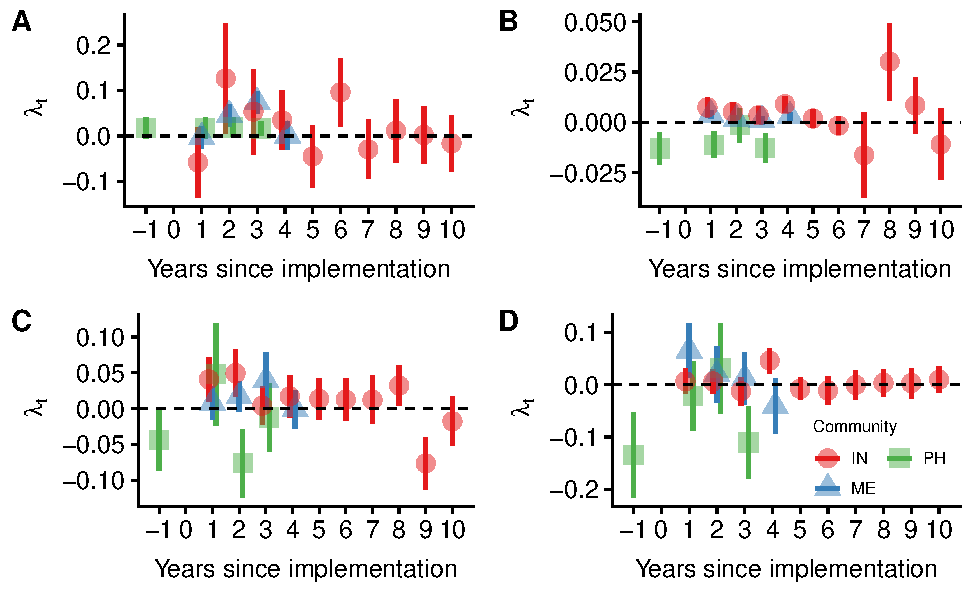
\includegraphics{Villasenor-Derbez_files/figure-latex/unnamed-chunk-8-1.pdf}
%DIF < DIFDELCMD < %%%
%DIFDELCMD < \DIFdelendFL \DIFaddbeginFL %%%
\DIFdelendFL 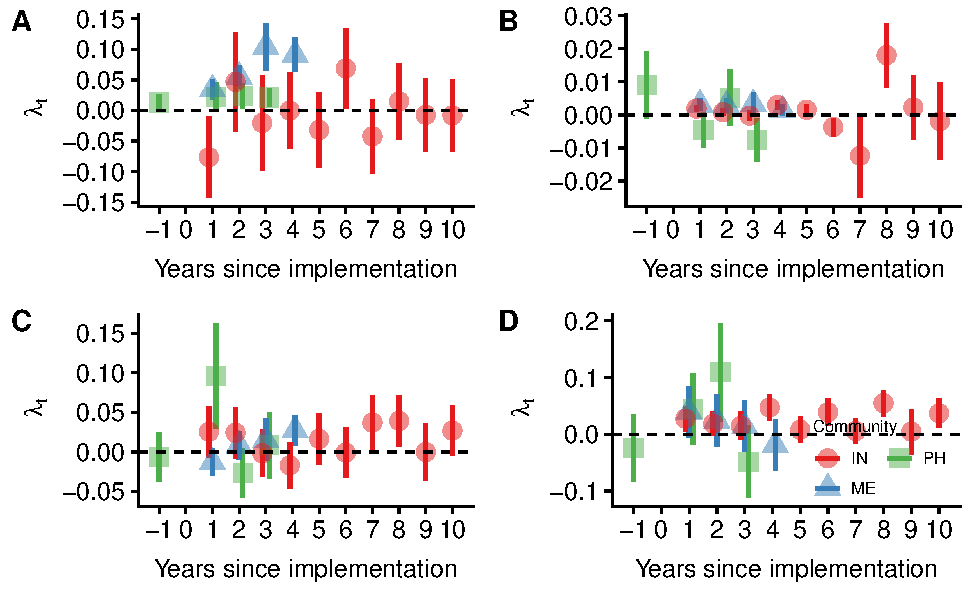
\includegraphics{manuscript_files/figure-latex/unnamed-chunk-8-1.pdf}
\DIFdelbeginFL %DIFDELCMD < \DIFaddendFL %%%
\DIFdelendFL \caption{\label{fig:unnamed-chunk-8}\label{fig:indicators}Effect sizes for
marine reserves from Isla Natividad (IN; red \DIFdelbeginFL %DIFDELCMD < \DIFdelbeginFL \DIFdelFL{cirlcles}\DIFdelendFL \DIFaddbeginFL \DIFaddFL{circles}\DIFaddendFL %%%
\DIFdelendFL \DIFaddbeginFL \DIFaddFL{circles}\DIFaddendFL ), Maria Elena (ME;
blue triangles), and Punta Herrero (PH; green squares) for lobster
densities (\emph{Panulirus spp}; A), fish biomass (B), invertebrate
densities (C), and fish densities (D). Plots are ordered by survey type
(left column: invertebrates; right column: fish). Points are jittered
hotizontally to avoid overplotting. Points indicate the effect size and
\DIFdelbeginFL %DIFDELCMD < \DIFaddbeginFL \DIFaddFL{error bars are heteroskedastic-robust }\DIFaddendFL %%%
\DIFdelendFL \DIFaddbeginFL \DIFaddFL{error bars are heteroskedastic-robust }\DIFaddendFL standard errors. Years have been
centered to year of implementation.}
\end{figure}

\begin{figure}
\centering
\DIFdelbeginFL %DIFDELCMD < \DIFdelbeginFL %%%
%DIF < DIFDELCMD < 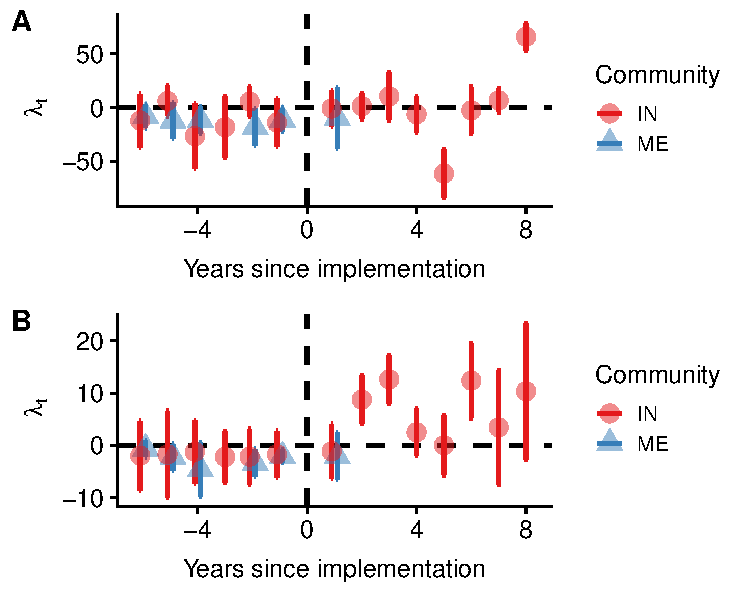
\includegraphics{Villasenor-Derbez_files/figure-latex/unnamed-chunk-9-1.pdf}
%DIF < DIFDELCMD < %%%
%DIFDELCMD < \DIFdelendFL \DIFaddbeginFL %%%
\DIFdelendFL 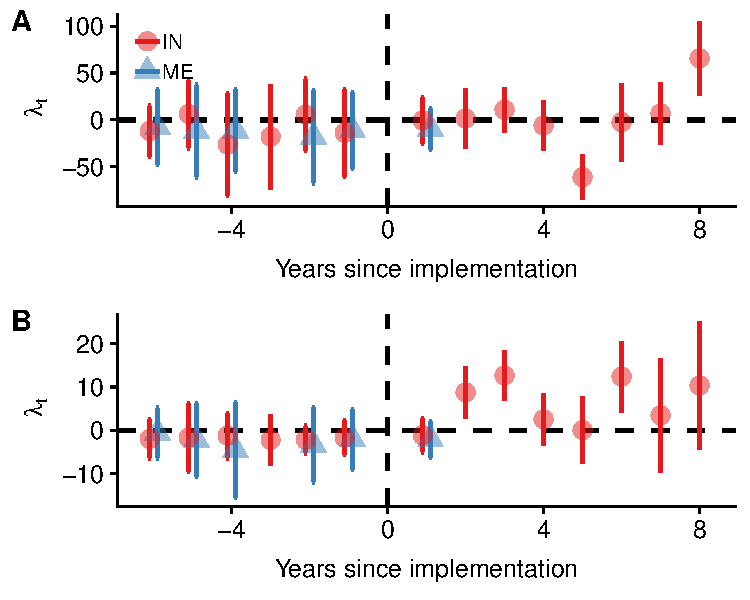
\includegraphics{manuscript_files/figure-latex/unnamed-chunk-9-1.pdf}
\DIFdelbeginFL %DIFDELCMD < \DIFaddendFL %%%
\DIFdelendFL \caption{\label{fig:unnamed-chunk-9}\label{fig:lobsters}Effect sizes for
lobster catches (A) and revenues (B) in at Isla Natividad (IN; red
circles) and Maria Elena (ME; blue triangles). Points \DIFdelbeginFL %DIFDELCMD < \DIFaddbeginFL \DIFaddFL{are jittered
%DIFDELCMD < hotizontally to avoid overplotting. Points }\DIFaddendFL %%%
\DIFdelendFL \DIFaddbeginFL \DIFaddFL{are jittered
hotizontally to avoid overplotting. Points }\DIFaddendFL indicate the effect size and
\DIFdelbeginFL %DIFDELCMD < \DIFaddbeginFL \DIFaddFL{error bars are heteroskedastic-robust }\DIFaddendFL %%%
\DIFdelendFL \DIFaddbeginFL \DIFaddFL{error bars are heteroskedastic-robust }\DIFaddendFL standard errors. Years have been
centered to year of implementation.}
\end{figure}

\begin{table}[H]

\caption{\label{tab:unnamed-chunk-10}\label{table:indicators}List of indicators used to evaluate the effectiveness of marine reserves, grouped by category.}
\centering
\begin{tabular}[t]{l|l}
\hline
Indicator & Units\\
\hline
\multicolumn{2}{l}{\textbf{Biological}}\\
\hline
\hspace{1em}Lobster density & org $\mathrm{m}^{-2}$\\
\hline
\hspace{1em}Invertebrate density & org $\mathrm{m}^{-2}$\\
\hline
\hspace{1em}Fish density & org $\mathrm{m}^{-2}$\\
\hline
\hspace{1em}Fish biomass & Kg $\mathrm{m}^{-2}$\\
\hline
\multicolumn{2}{l}{\textbf{Socioeconomic}}\\
\hline
\hspace{1em}Income from target species & M MXP\\
\hline
\hspace{1em}Landings from target species & Metric Tonnes\\
\hline
\end{tabular}
\end{table}

\begin{table}[H]

\caption{\label{tab:unnamed-chunk-11}\label{table:ses}Variables for the Social-Ecological System analysis (IN = Isla Natividad, ME = Maria Elena, PH = Punta Herrero). Alphanumeric codes follow \citet{basurto_2013-oq}; an asterisk (*) denotes variables incorporated based on \citet{difranco_2016-Xw} and \citet{edgar_2014-UO}. \DIFdelbeginFL %DIFDELCMD < \DIFaddbeginFL \DIFaddFL{The presented narrative applies equally for all communities unless otherwise noted.}\DIFaddendFL %%%
\DIFdelendFL \DIFaddbeginFL \DIFaddFL{The presented narrative applies equally for all communities unless otherwise noted.}\DIFaddendFL }
\centering
\DIFdelbeginFL %DIFDELCMD < \DIFdelbeginFL %%%
%DIF < DIFDELCMD < \resizebox{\linewidth}{!}{
%DIF < DIFDELCMD < \begin{tabular}[t]{>{\raggedright\arraybackslash}p{6.5cm}|>{\raggedright\arraybackslash}p{12cm}}
%DIF < DIFDELCMD < \hline
%DIF < DIFDELCMD < Variable & Narrative\\
%DIF < DIFDELCMD < \hline
%DIF < DIFDELCMD < \multicolumn{2}{l}{\textbf{Resource System (RS)}}\\
%DIF < DIFDELCMD < \hline
%DIF < DIFDELCMD < \hspace{1em}RS2 - Clarity of system boundaries: Clarity of geographical boundaries of TURF and reserves & Individual TURF and reserve boundaries are explicitly outlined in official documents that include maps and coordinates. Reserve placement is decided by the community. Fishers use GPS units and landmarks.\\
%DIF < DIFDELCMD < \hline
%DIF < DIFDELCMD < \hspace{1em}RS3 - Size of resource system: TURF Area (Km$^2$) & IN = 889.5; ME = 353.1; PH = 299.7\\
%DIF < DIFDELCMD < \hline
%DIF < DIFDELCMD < \hspace{1em}RS3 - Size of resource system: Reserve area (Evaluated reserve area; Km$^2$) & IN = 2 (1.3); ME = 10.48(0.09); PH = 11.25 (4.37)\\
%DIF < DIFDELCMD < \hline
%DIF < DIFDELCMD < \hspace{1em}RS4.1 - Stock status: Status of the main fishery & Lobster stocks are well managed, and are (IN) or have been (ME, PH) MSC certified.\\
%DIF < DIFDELCMD < \hline
%DIF < DIFDELCMD < \hspace{1em}*RS5 - Age of reserves: Years since reserves were implemented & IN = 12; ME = 6; PH = 5\\
%DIF < DIFDELCMD < \hline
%DIF < DIFDELCMD < \multicolumn{2}{l}{\textbf{Resource Unit (RU)}}\\
%DIF < DIFDELCMD < \hline
%DIF < DIFDELCMD < \hspace{1em}RU5 - Number of units (catch diversity): Number of targeted species & Lobster is their main fishery of these three communities, but they also target finfish. Additionally, fishers from Isla Natividad target other sedentary benthic invertebrates.\\
%DIF < DIFDELCMD < \hline
%DIF < DIFDELCMD < \multicolumn{2}{l}{\textbf{Actors (A)}}\\
%DIF < DIFDELCMD < \hline
%DIF < DIFDELCMD < \hspace{1em}A1 - Number of relevant actors: Number of fishers & IN = 98; ME = 80; PH = 21\\
%DIF < DIFDELCMD < \hline
%DIF < DIFDELCMD < \hspace{1em}*A3 - Isolation: Level of isolation of the fishing grounds & Their fishing grounds and reserves are highly isolated and away from dense urban centers.\\
%DIF < DIFDELCMD < \hline
%DIF < DIFDELCMD < \multicolumn{2}{l}{\textbf{Governance system (G)}}\\
%DIF < DIFDELCMD < \hline
%DIF < DIFDELCMD < \hspace{1em}GS6.1.4.3 - Territorial use communal rights : Presence of institutions that grant exclusive harvesting rights & Each community has exclusive access to harvest benthic resources, including lobster. These take the form of Territorial User Rights for Fisheries granted by the government to fishing cooperatives.\\
%DIF < DIFDELCMD < \hline
%DIF < DIFDELCMD < \hspace{1em}GS6.2 - Operational rules: Rules implemented by individuals atuhorized to partake on collective activities & Fishers have rules in addition to what the legislation mandates. These include larger minimum catch sizes, lower quotas, and assigning fishers to specific fishing grounds within their TURF.\\
%DIF < DIFDELCMD < \hline
%DIF < DIFDELCMD < \hspace{1em}GS9.1 - Social monitoring: Monitoring of the activities performed by cooperative members and external fishers & Fishing cooperatives have a group that monitors and enforces formal and internal rules. They ensure fishers of their fishing cooperative adhere to the established rules, and that foreign vessels do not poach their TURF and reserves.\\
%DIF < DIFDELCMD < \hline
%DIF < DIFDELCMD < \hspace{1em}GS9.2 - Biophysical monitoring: Monitoring of biological resources, including targeted species & Fishers perform annual standardized underwater surveys in the reserves and fishing grounds. Recently, they have installed oceanographic sensors to monitor oceanographic variables.\\
%DIF < DIFDELCMD < \hline
%DIF < DIFDELCMD < GS10.1 - Graduated sanctions & Fishers have penalties for breaking collective-choice rules or fishing inside the reserves. These may range from scoldings and warnings to not being allowed to harvest a particular resource or being expelled from the cooperative.\\
%DIF < DIFDELCMD < \hline
%DIF < DIFDELCMD < \end{tabular}}
%DIF < DIFDELCMD < %%%
%DIFDELCMD < \DIFdelendFL \DIFaddbeginFL %%%
\DIFdelendFL \resizebox{\linewidth}{!}{
\begin{tabular}[t]{>{\raggedright\arraybackslash}p{6.5cm}|>{\raggedright\arraybackslash}p{12cm}}
\hline
Variable & Narrative\\
\hline
\multicolumn{2}{l}{\textbf{Resource System (RS)}}\\
\hline
\hspace{1em}RS2 - Clarity of system boundaries: Clarity of geographical boundaries of TURF and reserves & Individual TURF and reserve boundaries are explicitly outlined in official documents that include maps and coordinates. Reserve placement is decided by the community. Fishers use GPS units and landmarks.\\
\hline
\hspace{1em}RS3 - Size of resource system: TURF Area (Km$^2$) & IN = 889.5; ME = 353.1; PH = 299.7\\
\hline
\hspace{1em}RS3 - Size of resource system: Reserve area (Evaluated reserve area; Km$^2$) & IN = 2 (1.3); ME = 10.48(0.09); PH = 11.25 (4.37)\\
\hline
\hspace{1em}RS4.1 - Stock status: Status of the main fishery & Lobster stocks are well managed, and are (IN) or have been (ME, PH) MSC certified.\\
\hline
\hspace{1em}*RS5 - Age of reserves: Years since reserves were implemented & IN = 12; ME = 6; PH = 5\\
\hline
\multicolumn{2}{l}{\textbf{Resource Unit (RU)}}\\
\hline
\hspace{1em}RU5 - Number of units (catch diversity): Number of targeted species & Lobster is their main fishery of these three communities, but they also target finfish (2 spp each). Additionally, fishers from Isla Natividad target other sedentary benthic invertebrates (4 spp).\\
\hline
\multicolumn{2}{l}{\textbf{Actors (A)}}\\
\hline
\hspace{1em}A1 - Number of relevant actors: Number of fishers & IN = 98; ME = 80; PH = 21\\
\hline
\hspace{1em}*A3 - Isolation: Level of isolation of the fishing grounds & Their fishing grounds and reserves are highly isolated and away from dense urban centers. IN lies 545 Km south from Tijuana, and ME and PH 230 Km south from Cancun, where the nearest international airports are located.\\
\hline
\multicolumn{2}{l}{\textbf{Governance system (G)}}\\
\hline
\hspace{1em}GS6.1.4.3 - Territorial use communal rights : Presence of institutions that grant exclusive harvesting rights & Each community has exclusive access to harvest benthic resources, including lobster. These take the form of Territorial User Rights for Fisheries granted by the government to fishing cooperatives.\\
\hline
\hspace{1em}GS6.2 - Operational rules: Rules implemented by individuals atuhorized to partake on collective activities & Fishers have rules in addition to what the legislation mandates. These are: larger minimum catch sizes, lower quotas, and assigning fishers to specific fishing grounds within their TURF.\\
\hline
\hspace{1em}GS9.1 - Social monitoring: Monitoring of the activities performed by cooperative members and external fishers & Fishing cooperatives have a group (Consejo de vigilancia) that monitors and enforces formal and internal rules. They ensure fishers of their fishing cooperative adhere to the established rules, and that foreign vessels do not poach their TURF and reserves.\\
\hline
\hspace{1em}GS9.2 - Biophysical monitoring: Monitoring of biological resources, including targeted species & Fishers perform annual standardized underwater surveys in the reserves and fishing grounds. Recently, they have installed oceanographic sensors to monitor oceanographic variables.\\
\hline
GS10.1 - Graduated sanctions & Fishers have penalties for breaking collective-choice rules or fishing inside the reserves. These may range from scoldings and warnings to not being allowed to harvest a particular resource or being expelled from the cooperative.\\
\hline
\end{tabular}}
\DIFdelbeginFL %DIFDELCMD < \DIFaddendFL %%%
\DIFdelendFL \end{table}



\end{document}